\chapter{Basics}
\label{sec:dd4hep-user-manual}

This chapter describes how supply a physics application developed with all the information related to the detector which is necessary to process data from particle collisions and to qualify the detecting apparatus in order to interpret these event data.

The clients of the detector description are the algorithms residing in the  event processing framework that need this information in order to perform their job (reconstruction, simulation, etc.). The detector description provided by DD4hep is a framework for developers to provide the specific detector information to software algorithms, which process data from particle collisions.

In the following sections an overview is given over the various independent elements of DD4hep followed by the discussion of an example which leads to  the description of a detector when combining these elements. This includes a discussion of the features of the DD4hep detector description and of its structure. 

\section{Building DD4hep}
\label{sec:dd4hep-user-manual-building}

The DD4hep source code is freely available and is distributed under the GPLv3 License. See the \texttt{doc/LICENSE} in the repository~\cite{dd4hep-repo} for more information. Please read the \textit{Release Notes} before downloading or using this release.

The DD4hep project consists of several packages. The idea  has been to separate the common parts of  the detector description toolkit from concrete detector examples. 

The package {\texttt{DDCore}} contains the definition of the basic classes of the toolkit: \texttt{Handle}, \texttt{DetElement}, \texttt{Volume}, \texttt{PlacedVolume}, \texttt{Shapes}, \texttt{Material}, etc. Most of these classes are \texttt{handles} to ROOT's TGeom classes.

\subsection{Supported Platforms}
\label{sec:dd4hep-user-manual-platforms}
Actively supported and tested platforms for DD4hep are :
\begin{itemize}
\item \texttt{Scientific Linux CERN 6}
\item \texttt{CERN CentOS 7}
\item \texttt{Apple macOS}
\end{itemize}
Support for any other platform will well be taken into account, but can only be actively supported by users who submit the necessary patches.

\subsection{Prerequisites}
\label{sec:dd4hep-user-manual-prerequisites}

DD4hep depends on a number of external packages. The user will need to install these in his/her system before building and running the examples
\begin{itemize}
\item \texttt{CMake} version 3.4 or higher 
\item \texttt{ROOT 6} installations.
\item \texttt{Xerces-C} if used to parse compact descriptions an installation of {Xerces-C} will is required.
\item To build DDG4 it is mandatory to have an installation of the \texttt{Boost} header files.
\item To build and run the simulation examples \texttt{Geant4} will be required. 
\end{itemize}

\subsection{CMake Build Options for DD4hep}
\label{sec:dd4hep-user-manual-building}

The package provides the basic mechanisms for constructing the \textit{Generic Detector Description Model} in memory from \texttt{XML} compact detector definition files. Two methods are currently supported: one based
on the \texttt{C++} \texttt{Xerces-C} parser.

The \texttt{XML} parsing method is enabled by default using the \texttt{TinyXML} parser. Optionally instead of \texttt{TinyXML} the \texttt{Xerces-C}  parser may be chosen by setting the two configuration options appropriately:

\begin{minted}[frame=single,framesep=3pt,breaklines=true,tabsize=2,linenos]{shell}
    -DDD4HEP_USE_XERCESC=ON
    -DXERCESC_ROOT_DIR=<path to Xerces-C-installation-directory>
\end{minted}

DDG4 is the package that contains the conversion of DD4hep geometry into Geant4 geometry to be used for simulation. The option \texttt{DD4HEP\_WITH\_GEANT4:BOOL} controls the building or not of this package that has the dependency to Geant4. The Geant4 installation needs to be located using the variable:

\begin{minted}[frame=single,framesep=3pt,breaklines=true,tabsize=2,linenos]{shell}
   -DDD4HEP_WITH_GEANT4=ON
   -DGeant4_DIR=<path to Geant4Config.cmake>
\end{minted}

To properly handle component properties using \texttt{boost::spirit}, access to the Boost header files must be provided.
\begin{minted}[frame=single,framesep=3pt,breaklines=true,tabsize=2,linenos,fontsize=\small]{bash}
    -DBoost_INCLUDE_DIR=<path to the boost include directory>
    -DBoost_NO_BOOST_CMAKE=ON  (to disable the search of boost-cmake)
\end{minted}

To build only the doxygen documentation and user manuals without the need for any dependencies one can use the following command
\begin{minted}[frame=single,framesep=3pt,breaklines=true,tabsize=2,linenos]{shell}
  cmake -DBUILD_DOCS_ONLY=ON ..
\end{minted}
After one can execute the following target for building doxygen documentation
\begin{minted}[frame=single,framesep=3pt,breaklines=true,tabsize=2,linenos]{shell}
make reference
\end{minted}
and for building the user manuals
\begin{minted}[frame=single,framesep=3pt,breaklines=true,tabsize=2,linenos]{shell}
make pdf
\end{minted}

\subsection{Build From Source}
\label{sec:dd4hep-user-manual-building-from-source}
NEED REWRITE ONCE FINALIZED
%The following steps are necessary to build DD4hep:
%\begin{itemize}
%\item Set the environment, at least ROOT needs to be initialized, e.g.
%    \begin{minted}[frame=single,framesep=3pt,breaklines=true,tabsize=2,linenos,fontsize=\small]{bash}
%      source  /data/ilcsoft/root/5.34.03/bin/thisroot.sh
%    \end{minted}
%    \vspace{-0.6cm}
%   (the bare minimum is: \texttt{export ROOTSYS=<path to root installation>}).
%
%\item First checkout code from the repository:
%    \begin{minted}[frame=single,framesep=3pt,breaklines=true,tabsize=2,linenos,fontsize=\small]{bash}
%      svn co https://svnsrv.desy.de/public/aidasoft/DD4hep/trunk DD4hep
%    \end{minted}
%    \vspace{-0.6cm}
%
%\item We refer to the directory DD4hep as the source directory. The 
%next step is to create a directory in which to configure and run the build 
%and store the build products. This directory should not be the same as, or 
%inside, the source directory. In this guide, we create this build directory 
%alongside our source directory: 
%\begin{minted}[frame=single,framesep=3pt,breaklines=true,tabsize=2,linenos]{cmake}
%      mkdir build
%      cd build
%      cmake -DCMAKE_INSTALL_PREFIX=<dd4hep-install-pasth> <CMake-options> ../DD4hep
%      make -j 4
%      make install
%    \end{minted}
%\end{itemize}
%The CMake Variable \texttt{CMAKE\_INSTALL\_PREFIX} is used to set the install directory, 
%the directory under which the DD4hep libraries, headers and support files 
%will be installed.


\subsection{Remarks}
\label{sec:dd4hep-user-manual-remarks}
The main reference is the doxygen information of DD4hep and the ROOT documentation. Please refer to these sources for a detailed view of the capabilities of each component and/or its handle. For coherence reasons, the description of the interfaces is limited to examples which illustrate the usage of the basic components. 

\subsection{Caveat}
\label{sec:dd4hep-user-manual-caveat}
NEEDS ADDITIONAL CLARIFICATION
%The atomic units in of Geant4 are (millimeter, nanosecond and MeV and radians).
%The atomic units of ROOT-TGeo are (centimeter, seconds, GeV and degrees).
%Unfortunately the authors could not agree on a common system of units
%and mixing the two can easily result in a chaos.
%Users must be aware of this fact.

\section{DD4hep Handles}
\label{sec:dd4hep-user-manual-handles}

Handles are the means of clients accessing DD4hep detector description data. Handles are an intrinsic ingredient to DD4hep meant to also support various views onto relatively simple structures. The data itself is not held by the handle itself, the handle only allows the access to the data typically held by a pointer.

DD4hep internally prefers to expose data structures which are as simple as possible while at the same time being as complicated as necessary. These objects are then manipulated by Handles, smart pointer objects with sometimes specialized functionality depending on the contained data type. It is seen as a clear advantage that these smart pointer objects to not impose any restrictions on the underlying object except the accessibility of the contained data.

The freedom to attach handle based facades to virtually any data item allows for optimized data views depending on the application type, such as special views for reconstruction, simulation, tracking, etc.

For the importance of the functionality of this issue we repeat here the functionality described in~\ref{subsect:extesions-and-views} which is achieved by specializing the basic templated handle implementation:
\begin{description}
\item [Convenience Views] provide higher level abstractions and internally group complex calculations. Such views simplify the life of the end-users.
\item [Optimization Views] allows end-users extend the data of the common detector detector element and store precomputed results, which would be expensive to obtain repeatedly.
\item [Compatibility Views] help to ensure smooth periods of software redesign. During the life-time of the experiment often various software constructs are for functional reasons re-designed and re-engineered. Compatibility Views either adapt new data designs to existing application code or expose new behavior based on existing data.
\end{description}

Since the lifetime of DD4hep objects is mostly defined by the lifetime of the {\texttt{dd4hep::Detector}} object (in turn defining the lifetime of ROOT's {\texttt{TGeoManager}}) or for the conditions is managed by the ConditionsManager object under the steering of the embedding framework there is also no memory model imposed which would only lead to performance penalties. Hence, handles can be applied to data structures independent of their origin:
\begin{itemize}
\item allocated from the stack
\item allocated from the heap
\item allocated as single objects of in bulk by array constructors.
\end{itemize}

There is no restriction to allow toolkit users to extend any of the internally used DD4hep classes such as e.g. the {\texttt{dd4hep::DetElement}} data object {\texttt{dd4hep::detail::DetElementObject}} with their own implementation supporting further enhanced functionality both in terms of additional data and additional member functions provided the user specialized class inherits from the DD4hep provided base. Obviously such enhancements do not hold for the geometry classes provided by ROOT because here the ROOT framework internally calls its object constructors. Hence, though DD4hep internally uses templated handles to manipulate data objects, DD4hep allows for all freedom to extend any of the internally used objects and a priori no restrictions are imposed by the DD4hep framework besides the mentioned inheritance.

The design approach of DD4hep to internally use handles to manipulate objects which is also offered to clients clearly has difficulties to support the Liskov substitution principle. This was a conscious decision when designing DD4hep.

Frameworks which see the substitution principle for the implementation of the simple data structures mandatory for its functionality clearly limit the  benefits of the handles unless

\begin{itemize}
\item the depending frameworks provides handles which are a fully implemented facade or
\item the depending framework use consistently the operator->() provided by all   handles to directly access the underlying object or
\item the depending framework uses DD4hep and it is provided only internally and provide top level user code only with pointers/references to the data structures in their full object oriented glory.
\end{itemize}

The template handle class (see for details the \href{https://dd4hep.web.cern.ch/dd4hep/reference/classdd4hep_1_1Handle.html}{\texttt{Handle.h}} header file) allows type safe assignment of other unrelated handles and supports standard data conversions to the underlying object in form of the raw pointer, a reference etc.
The template handle class:

\begin{minted}[frame=single,framesep=3pt,breaklines=true,tabsize=2,linenos,fontsize=\small]{c++}
template <typename T> class Handle {
public:
  // Type definitions and class specific abbreviations and forward declarations
  typedef T Implementation;
  typedef Handle<Implementation> handle_t;
public:
  // Single and only data member: pointer to the underlying object
  T* m_element;
public:
  Handle() : m_element(0) { }
  Handle(T* e) : m_element(e) { }
  Handle(const Handle<T>& e) : m_element(e.m_element) { }
  template<typename Q> Handle(Q* e) : m_element((T*)e) { verifyObject(); }
  template<typename Q> Handle(const Handle<Q>& e) : m_element((T*)e.m_element) { verifyObject(); }
  Handle<T>& operator=(const Handle<T>& e) { m_element=e.m_element; return *this;}
  bool isValid() const { return 0 != m_element; }
  bool operator!() const { return 0 == m_element; }
  void clear() { m_element = 0; }
  T* operator->() const { return m_element; }
  operator T& () const { return *m_element; }
  T& operator*() const { return *m_element; }
  T* ptr() const { return m_element; }
  template <typename Q> Q* _ptr() const { return (Q*)m_element; }
  template <typename Q> Q* data() const { return (Q*)m_element; }
  template <typename Q> Q& object() const { return *(Q*)m_element; }
  const char* name() const;
};
\end{minted}
effectively works like a pointer with additional object validation during assignment and construction. Handles support direct access to the held object: either by using the 
\begin{minted}[frame=single,framesep=3pt,breaklines=true,tabsize=2,fontsize=\small]{c++}
       operator->()                        (See line 19 above)
\end{minted}
or the automatic type conversions:
\begin{minted}[frame=single,framesep=3pt,breaklines=true,tabsize=2,fontsize=\small]{c++}
      operator T& ()  const                (See line 20-21 above)
      T& operator*()  const
\end{minted}

All entities of the DD4hep detector description are exposed as handles - raw pointers should not occur in the code. The handles to these objects serve two purposes:
\begin{itemize}
\item Hold a pointer to the object and extend the functionality of a raw pointer.
\item Enable the creation of new objects using specialized constructors within sub-classes. To ensure memory integrity and avoid resource  leaks these created objects should always be stored in the detector description data hub \texttt{Detector} described in section~\ref{sec:dd4hep-user-manual-LCDD-hub}.
\end{itemize}


\section{The Data Extension Mechanism}
\label{sec:dd4hep-user-manual-data-extensions}

Data extensions are client defined \texttt{C++} objects aggregated to basic DD4hep objects. The need to introduce such data extensions results from the simple fact that no data structure can be defined without the iterative need in the long term to extend it leading to implementations, which can only satisfy a subset of possible clients. To accomplish for this fact a mechanism was put in place which allows any user to attach any supplementary information provided the information is embedded in a polymorph object with an accessible destructor. There is one limitation though: object extension must differ by their interface type. There may not be two objects attached with the identical interface type. The actual implemented sub-type of the extension is not relevant. Separating the interface type from the implementation type keeps client code still functional even if the implementation of the extension changes 
or is a plug-able component.

The following code snippet shows the extension interface:

\begin{minted}[frame=single,framesep=3pt,breaklines=true,tabsize=2,linenos,fontsize=\small]{c++}
  /// Extend the object with an arbitrary structure accessible by the type
  template <typename IFACE, typename CONCRETE> IFACE* addExtension(CONCRETE* c);
  /// Access extension element by the type
  template <class T> T* extension() const;
\end{minted}

Assuming a client class of the following structure:
\begin{minted}[frame=single,framesep=3pt,breaklines=true,tabsize=2,linenos,fontsize=\small]{c++}
  class ExtensionInterface {
    virtual ~ExtensionInterface();
    virtual void foo() = 0;
  };

  class ExtensionImplementation : public ExtensionInterface {
    ExtensionImplementation();
    virtual ~ExtensionImplementation();
  virtual void foo();
  };
\end{minted}
is then attached to an extensible object as follows:
\begin{minted}[frame=single,framesep=3pt,breaklines=true,tabsize=2,linenos,fontsize=\small]{c++}
  ExtensionImplementation* ptr = new ExtensionImplementation();
  /// ... fill the ExtensionImplementation instance with data ...
  module.addExtension<ExtensionInterface>(ptr);
\end{minted}
The data extension may then be retrieved whenever the instance of the extensible object ``module'' is accessible:
\begin{minted}[frame=single,framesep=3pt,breaklines=true,tabsize=2,linenos,fontsize=\small]{c++}
  ExtensionInterface* ptr = module.extension<ExtensionInterface>();
\end{minted}
The look-up mechanism is rather efficient. Though it is advisable to cache the pointer within the client code if the usage is very frequent.

There are currently three object types present which support this mechanism:
\begin{itemize}
\item the central object of DD4hep, the \texttt{Detector} class discussed in section~\ref{sec:dd4hep-user-manual-LCDD-hub}.
\item the object describing subdetectors or parts thereof, the \texttt{DetElement} class discussed in section~\ref{sec:dd4hep-user-manual-detector-elements}. Detector element extensions in addition require the presence of a copy constructor to support e.g. reflection operations. Without a copy mechanism detector element hierarchies could cloned.
\item the object describing sensitive detectors, the \texttt{SensitiveDetector} class discussed in section~\ref{sec:dd4hep-user-manual-sensitive-detectors}.
\end{itemize}

\section{XML Tools and Interfaces}
\label{sec:dd4hep-user-manual-xml-tools}

Using native tools to interpret \texttt{XML} structures is rather tedious and lengthy. To easy the access to \texttt{XML} data considerable effort was put in place to easy the life of clients as much as possible using predefined instructs to access \texttt{XML} attributes, elements or element collections.

The functionality of the \texttt{XML} tools is perhaps best shown with a small example. Imagine to extract the data from an \texttt{XML} snippet like the following:
\begin{minted}[frame=single,framesep=3pt,breaklines=true,tabsize=2,linenos,fontsize=\small]{xml}
  <detector name="Something">
    <tubs rmin="BP_radius - BP_thickness" rmax="BP_radius" zhalf="Endcap_zmax/2.0"/>
    <position x="0" y="0" z="Endcap_zmax/2.0" />
    <rotation x="0.0" y="CrossingAngle/2.0" z="0.0" />
    <layer id="1" inner_r="Barrel_r1" outer_r="Barrel_r1 + 0.02*cm" inner_z="Barrel_zmax + 0.1*cm">
      <slice material = "G10" thickness ="0.5*cm"/>
    </layer>
    <layer id="2" inner_r="Barrel_r2" outer_r="Barrel_r2 + 0.02*cm" inner_z="Barrel_zmax + 0.1*cm">
     <slice material = "G10" thickness ="0.5*cm"/>
    </layer>
    ....
  </detector>
\end{minted}

The variable names used in the \texttt{XML} snippet are evaluated when interpreted. Unless the attributes are accessed as strings, the client never sees the strings, but only the evaluated numbers. The anatomy of the \texttt{C++} code snippets to interpret such a data section looks very similar:
\begin{minted}[frame=single,framesep=3pt,breaklines=true,tabsize=2,linenos,fontsize=\small]{c++}
  static void some_xml_handler(xml_h e)  {
    xml_det_t  x_det  (e);
    xml_comp_t x_tube    = x_det.tubs();
    xml_dim_t  pos       = x_det.position();
    xml_dim_t  rot       = x_det.rotation();
    string     name      = x_det.nameStr();
      
    for(xml_coll_t i(x_det,_U(layer)); i; ++i)  {
      xml_comp_t x_layer = i;
      double  zmin = x_layer.inner_z();
      double  rmin = x_layer.inner_r();
      double  rmax = x_layer.outer_r();
      double  layerWidh = 0;
        
      for(xml_coll_t j(x_layer,_U(slice)); j; ++j)  {
        double thickness = xml_comp_t(j).thickness();
        layerWidth += thickness;
      }
    }
  }
\end{minted}
In the above code snippet an \texttt{XML} (sub-)tree is passed to the executing function as a handle to an \texttt{XML} element ({\texttt{xml\_h}}). Such handles may seamlessly be assigned to any supporting helper class inheriting from the class {\texttt{XML::Element}}, which encapsulates the functionality required to interpret the \texttt{XML} structures. Effectively the various \texttt{XML} attributes and child nodes are accessed using functions with the same name from a convenience handle. In lines 3-5 child nodes are extracted, lines 10-12,16 access element attributes.Element collections with the same tag names \texttt{layer} and \texttt{slice} are exposed to the client code using an iteration mechanism.

Note the macros \texttt{\_U(layer)} and \texttt{\_U(slice)}:  When using \texttt{Xerces-C} as an \texttt{XML} parser, it will expand to the reference to an object containing the unicode value of the string ``layer''. The full list of predefined tag names can be found in the include file \texttt{XML/UnicodeValues.h}. If a user tag is not part in the precompiled tag list, the corresponding Unicode string may be created with the macro \texttt{\_Unicode(layer)} or the function \texttt{Unicode(``layer'')}.

The convenience handles actually implement these functions to ease life. There is no magic - newly created attributes with new names obviously cannot be accessed with convenience mechanism. Hence, either you know what you are doing and you create your own convenience handlers or you restrict yourself a bit in the creativity of defining new attribute names.

There exist several utility classes to extract data from predefined \texttt{XML} tags:
\begin{itemize}
\item Any \texttt{XML} element is described by an \texttt{XML} handle \texttt{\texttt{XML::Handle\_t}} ({\texttt{xml\_t}}). Handles are the basic structure for the support of higher level interfaces described above. The assignment of a handle to any of the interfaces below is possible.
\item The class \texttt{\texttt{XML::Element}} ({\texttt{xml\_elt\_t}}) supports in a simple way the navigation through the hierarchy of the \texttt{XML} tree accessing child nodes and attributes. Attributes at this level are named entities and the tag name must be supplied.
\item The class \texttt{\texttt{XML::Dimension}} with the type definition {\texttt{xml\_dim\_t}}, supports numerous access functions named identical to the
\texttt{XML} attribute names. Such helper classes simplify the tedious string handling required by the 
\item The class \texttt{\texttt{XML::Component}} ({\texttt{xml\_comp\_t}}) and the class \texttt{\texttt{XML::Detector}} ({\texttt{xml\_det\_t}}) resolving other issues useful to construct detectors.
\item Sequences of \texttt{XML} elements with an identical tag name may be handled as iterations as shown in the Figure above using the class \texttt{\texttt{XML::Collection\_t}}.
\item Convenience classes, which allow easy access to element attributes  may easily be constructed using the methods of the {\texttt{XML::Element}} class. This allows to construct very flexible thou non-intrusive extensions to DD4hep. Hence there is a priori no need to modify these helpers for the benefit of only one single client. In the presence of multiple requests such extensions may though be adopted.
\end{itemize}
It is clearly the responsibility of the client to only request attributes from an \texttt{XML} element, which exist. If an attribute, a child node etc. is not found within the element an exception is thrown.

The basic interface of the \texttt{XML::Element} class allows to access tags and child nodes not exposed by the convenience wrappers:
\begin{minted}[frame=single,framesep=3pt,breaklines=true,tabsize=2,linenos,fontsize=\small]{c++}
  /// Access the tag name of this DOM element
  std::string tag() const;
  /// Access the tag name of this DOM element
  const XmlChar* tagName() const;

  /// Check for the existence of a named attribute
  bool hasAttr(const XmlChar* name) const;
  /// Retrieve a collection of all attributes of this DOM element
  std::vector<Attribute> attributes() const;
  /// Access single attribute by its name
  Attribute getAttr(const XmlChar* name) const;
  /// Access attribute with implicit return type conversion
  template <class T> T attr(const XmlChar* tag) const;
  /// Access attribute name (throws exception if not present)
  const XmlChar* attr_name(const Attribute attr) const;
  /// Access attribute value by the attribute  (throws exception if not present)
  const XmlChar* attr_value(const Attribute attr) const;

  /// Check the existence of a child with a given tag name
  bool hasChild(const XmlChar* tag) const;
  /// Access child by tag name. Thow an exception if required in case the child is not present
  Handle_t child(const Strng_t& tag, bool except = true) const;
  /// Add a new child to the DOM node
  Handle_t addChild(const XmlChar* tag) const;
  /// Check if a child with the required tag exists - if not create it and add it to the current node
  Handle_t setChild(const XmlChar* tag) const;
\end{minted}

\section{The Detector Description Data Hub: \texttt{Detector}}
\label{sec:dd4hep-user-manual-LCDD-hub}
As shown in Figure~\ref{fig:dd4hep-detector-model}, any access to the detector  description data is done using a standardized interface called \texttt{Detector}. During the configuration phase of the detector the interface is used to populate the internal data structures. Data structures present in the memory layout of the detector description may be retrieved by clients at any time using the  \href{https://dd4hep.web.cern.ch/dd4hep/reference/classdd4hep_1_1Detector.html}{\texttt{Detector} interface class}. This includes of course, the access during the actual detector construction. The following code listing shows the accessor method to retrieve  detector description entities from the interface. Not shown are access methods for groups of these entities and the methods to add objects:

\begin{minted}[frame=single,framesep=3pt,breaklines=true,tabsize=2,linenos,fontsize=\small]{c++}
class Detector {
  ///+++ Shortcuts to access often used quantities

  /// Return handle to material describing air
  virtual Material air() const = 0;
  /// Return handle to material describing vacuum
  virtual Material vacuum() const = 0;
  /// Return handle to "invisible" visualization attributes
  virtual VisAttr invisible() const = 0;

  ///+++ Access to the top level detector elements and the corresponding volumes

  /// Return reference to the top-most (world) detector element
  virtual DetElement world() const = 0;
  /// Return reference to detector element with all tracker devices.
  virtual DetElement trackers() const = 0;

  /// Return handle to the world volume containing everything
  virtual Volume worldVolume() const = 0;
  /// Return handle to the volume containing the tracking devices
  virtual Volume trackingVolume() const = 0;

  ///+++ Access to geometry and detector description objects

  /// Retrieve a constant by its name from the detector description
  virtual Constant constant(const std::string& name)      const = 0;
  /// Retrieve a matrial by its name from the detector description
  virtual Material material(const std::string& name)      const = 0;
  /// Retrieve a field component by its name from the detector description
  virtual DetElement detector(const std::string& name)      const = 0;
  /// Retrieve a sensitive detector by its name from the detector description
  virtual SensitiveDetector sensitiveDetector(const std::string& name) const = 0;
  /// Retrieve a readout object by its name from the detector description
  virtual Readout readout(const std::string& name)       const = 0;
  /// Retrieve a id descriptor by its name from the detector description
  virtual IDDescriptor idSpecification(const std::string& name)   const = 0;
  /// Retrieve a subdetector element by its name from the detector description
  virtual CartesianFieldfield(const std::string& name)     const = 0;

  ///+++ Access to visualisation attributes and Geant4 processing hints

  /// Retrieve a visualization attribute by its name from the detector description
  virtual VisAttr visAttributes(const std::string& name) const = 0;

  /// Retrieve a region object by its name from the detector description
  virtual Region  region(const std::string& name)    const = 0;
  /// Retrieve a limitset by its name from the detector description
  virtual LimitSet limitSet(const std::string& name)      const = 0;
  //...
  
  ///+++ Extension mechanism:
  /// Extend the sensitive detector element with an arbitrary structure accessible by the type
  template <typename IFACE, typename CONCRETE> IFACE* addExtension(CONCRETE* c)
};
\end{minted}

As shown in the above listing, the \texttt{Detector} interface is the main access point to access a whole set 
\begin{itemize}
\item often used predefined values such as the material ``air'' or ``vacuum'' (line 5--10).
\item the top level objects ``world'', ``trackers'' and the corresponding volumes (line 14--21).
\item items in the constants table containing named definitions also used during the interpretation of the \texttt{XML} content after parsing (line 26)
\item named items in the the material table (line 28)
\item named subdetectors after construction and the corresponding (line 30)
\item named sensitive detectors with their (line 32)
\item named readout structure definition using a (line 34)
\item named readout identifier descriptions (line 36)
\item named descriptors of electric and/or magnetic fields  (line 39).
\end{itemize}
Additional support for specialized applications is provided by the interface:
\begin{itemize}
\item Geant4: named region settings  (line 46)
\item Geant4: named limits settings  (line 48)
\item Visualization: named visualization attributes  (line 43)
\item User defined extensions (line 53) are supported with the extension mechanism described in section~\ref{sec:dd4hep-user-manual-data-extensions}.
\end{itemize}

All the values are populated either directly from \texttt{XML} or from \textit{detector constructors} (see section~\ref{sec:detector-constructors}). The interface also allows to load \texttt{XML} configuration files of any kind provided an appropriate  interpretation plugin is present. In the next section we describe the functionality  of the ``lccd'' plugin used to interpret the compact detector description. This mechanism can easily be extended using ROOT plugins, where the plugin name must correspond to the \texttt{XML} root element of the document to be interpreted.

\section{Detector Description Persistency in \texttt{XML}}
\label{sec:compact-xml-structure}
As explained in a previous section, the mechanism involved in the data loading  allow an application to be fairly independent of the technology used to populate the transient detector representation. However, if one wants to use a given technology, she/he has to get/provide the corresponding conversion mechanism. The choice of \texttt{XML} was driven mainly by its easiness of use and the number of tools provided for its manipulation and parsing. Moreover, \texttt{XML} data can be easily translated into many other format using tools like \texttt{XSLT}  processors. The grammar used for the \texttt{XML} data is pretty simple and straight forward, actually very similar to other geometry description languages based on \texttt{XML}. For example the material description is nearly identical to the material description in \texttt{GDML}~\cite{Chytracek:2006be}. The syntactic structure of the compact \texttt{XML} description was taken from the SiD detector description~\cite{Gaede:81331}. The following listing shows the basic layout of any the compact detector description file with its different sections:

\begin{minted}[frame=single,framesep=3pt,breaklines=true,tabsize=2,linenos,fontsize=\small]{xml}
<lccdd>
  <info>   ...    </info>       Auxiliary detector model information
  <includes>  ... </includes>   Section defining GDML files to be included
  <define>  ...   </define>     Dictionary of constant expressions and variables
  <materials> ... </materials>  Additional material definitions
  <display>  ...  </display>    Definition of visualization attributes
  <detectors> ... </detectors>  Section with sub-detector definitions
  <readouts>  ... </readouts>   Section with readout structure definitions
  <limits>  ...   </limits>     Definition of limit sets for Geant4
  <fields>  ...   </fields>     Field definitions
</lccdd>
\end{minted}

The root tag of the \texttt{XML} tree is {\texttt{lccdd}}. This name is fixed. In the following the content of the various sections is discussed. The \texttt{XML} sections are filled with the following information:
\begin{itemize}
\item {\textbf{The \texttt{<info>} sub-tree}} contains auxiliary information about the detector model:
\begin{minted}[frame=single,framesep=3pt,breaklines=true,tabsize=2,linenos,fontsize=\small]{xml}
<info name="clic_sid_cdr"
  title="CLIC Silicon Detector CDR"
  author="Christian Grefe"
  url="https://twiki.cern.ch/twiki/bin/view/CLIC/ClicSidCdr"
  status="development"
  version="$Id: compact.xml 665 2013-07-02 18:49:26Z markus.frank $">
  <comment>The compact format for the CLIC Silicon Detector used 
           for the conceptual design report</comment>
</info>
\end{minted}

\item {\textbf{The \texttt{<includes>} section}} allows to include GDML sub-trees containing material descriptions. These files are processed {\textit{before}} the detector constructors are called:
\begin{minted}[frame=single,framesep=3pt,breaklines=true,tabsize=2,linenos,fontsize=\small]{xml}
<includes>
  <file  ref="elements.xml"/>
  <file  ref="materials.xml"/>
   ...
</includes>
\end{minted}
For historic reasons the tag {\textbf{\texttt{<gdmlFile>}}} is supported but deprecated in parallel
with the new tag {\textbf{\texttt{<file>}}}.


\item {\textbf{The \texttt{<define>} section}} contains all variable definitions defined by the client to simplify the definition of subdetectors. These name-value pairs are fed to the expression evaluator and must evaluate by default to a number. The data type
  {\texttt{number}} is assumed by default (see example below).
These {\texttt{number}} variables can be combined to formulas e.g. to automatically re-dimension subdetectors if boundaries are changed:
\begin{minted}[frame=single,framesep=3pt,breaklines=true,tabsize=2,linenos,fontsize=\small]{xml}
<define>
  <constant name="world_side" value="30000" type="number"/>
  <constant name="world_x" value="world_side"/>
  <constant name="world_y" value="world_side"/>
  <constant name="world_z" value="world_side"/>
  ....
</define>
\end{minted}
The other allowed data type is {\texttt{string}}. {\texttt{string}} values are stored in the raw format in the {\texttt{Detector}} object instance and can be retrieved by name. The values are as well added to the evaluation dictionary in order to resolve e.g. environment paths.

\item  {\textbf{The \texttt{<materials>} sub-tree}} contains additional materials, which are not contained in the default materials tables. The snippet below shows an example to extend the table of known materials. For more details please see section~\ref{sec:compact-material-description}.
\begin{minted}[frame=single,framesep=3pt,breaklines=true,tabsize=2,linenos,fontsize=\small]{xml}
<materials>
  <!-- The description of an atomic element or isotope -->
  <element Z="30" formula="Zn" name="Zn" >
    <atom type="A" unit="g/mol" value="65.3955" />
  </element>
  ...
  <!-- The description of a new material               -->
  <material name="CarbonFiber_15percent">
    ...
  </material>
  ...
</materials>
\end{minted}

\item {\textbf{The visualization attributes}} are defined in the \texttt{<display>} section. Clients access visualization settings by name. The possible attributes are shown below and essentially contain the RGB color values, the visibility and the drawing style:
\begin{minted}[frame=single,framesep=3pt,breaklines=true,tabsize=2,linenos,fontsize=\small]{xml}
<display>
  <vis name="InvisibleNoDaughters"      
       showDaughters="false" 
       visible="false"/>
  <vis name="SiVertexBarrelModuleVis" 
       alpha="1.0" r="1" g="1" b="0.6" 
       drawingStyle="solid" 
       showDaughters="true" 
       visible="true"/>
  ....
</display>
\end{minted}

\item {\textbf{<Limisets>}} contain parameters passed to Geant4:
\begin{minted}[frame=single,framesep=3pt,breaklines=true,tabsize=2,linenos,fontsize=\small]{xml}
<limits>
    <limitset name="cal_limits">
        <limit name="step_length_max" particles="*" value="5.0" unit="mm" />
    </limitset>
</limits>
\end{minted}

\item {\textbf{The \texttt{detectors}}} section contains subtrees of the type \texttt{<detector>} which contain all parameters used by the \textit{detector constructors} to actually expand the geometrical structure. Each subdetector has a name and a type, where the type is used to call the proper constructor plugin. If the subdetector element is sensitive, a forward reference to the corresponding readout structure is mandatory. The remaining parameters are user defined:

\begin{minted}[frame=single,framesep=3pt,breaklines=true,tabsize=2,linenos,fontsize=\small]{xml}
<detectors>
  <detector id="4" name="SiTrackerEndcap" type="SiTrackerEndcap" readout="SiTrackerEndcapHits">
    <comment>Outer Tracker Endcaps</comment>
    <module name="Module1" vis="SiTrackerEndcapModuleVis">
      <trd x1="36.112" x2="46.635" z="100.114/2" />
      <module_component thickness="0.00052*cm"   material="Copper" />
      <module_component thickness="0.03*cm"   material="Silicon" sensitive="true" />
      ...
    </module> 
    ...
    <layer id="1">
      <ring r="256.716" zstart="787.105+1.75" nmodules="24" dz="1.75" module="Module1"/>
      <ring r="353.991" zstart="778.776+1.75" nmodules="32" dz="1.75" module="Module1"/>
      <ring r="449.180" zstart="770.544+1.75" nmodules="40" dz="1.75" module="Module1"/>
    </layer>
    ...
  </detector>
</detectors>
\end{minted}

\item {\textbf{The \texttt{<readouts>} section}} defined the encoding of sensitive volumes to so-called cell-ids, which are in DD4hep 64-bit integer numbers. The encoding is subdetector dependent with one exception: to uniquely identity each subdetector, the width of the system field must be the same.
\begin{minted}[frame=single,framesep=3pt,breaklines=true,tabsize=2,linenos,fontsize=\small]{xml}
<readouts>
  <readout name="SiTrackerEndcapHits">
    <id>system:8,barrel:3,layer:4,module:14,sensor:2,side:32:-2,strip:20</id>
  </readout>
  ...
</readouts>
\end{minted}

\item {\textbf{Electromagnetic fields}} are described in the \texttt{<fields>} section. There may be several fields present. In DD4hep the resulting field vectors
may be both electric and magnetic. The strength of the overall field is calculated as the superposition of the individual components:
\begin{minted}[frame=single,framesep=3pt,breaklines=true,tabsize=2,linenos,fontsize=\small]{xml}
<fields>
  <field name="GlobalSolenoid" type="solenoid" 
         inner_field="5.0*tesla"
         outer_field="-1.5*tesla" 
         zmax="SolenoidCoilOuterZ"
         outer_radius="SolenoidalFieldRadius">
  </field>
  ...
</fields>
\end{minted}
\end{itemize}

\section{Units}
DD4hep offers the user the possibility to choose and use the preferred units for any quantity and offers a consistent units solution defined as:
\begin{minted}[frame=single,framesep=3pt,breaklines=true,tabsize=2,linenos,fontsize=\small]{c++}
static constexpr double centimeter = 1.;
static constexpr double second = 1.;
static constexpr double kiloelectronvolt = 1;
static constexpr double eplus = 1.;
static constexpr double kelvin = 1.;
static constexpr double mole = 1.;
static constexpr double candela = 1.;
static constexpr double radian = 1.;
static constexpr double steradian = 1.;
\end{minted}
All other units are derived from the base ones:
\begin{minted}[frame=single,framesep=3pt,breaklines=true,tabsize=2,linenos,fontsize=\small]{c++}
static constexpr double centimeter = 10. * millimeter;
static constexpr double centimeter2 = centimeter * centimeter;
static constexpr double centimeter3 = centimeter * centimeter * centimeter;

static constexpr double meter = 1000. * millimeter;
static constexpr double meter2 = meter * meter;
static constexpr double meter3 = meter * meter * meter;

static constexpr double kilometer = 1000. * meter;
static constexpr double kilometer2 = kilometer * kilometer;
static constexpr double kilometer3 = kilometer * kilometer * kilometer;

static constexpr double kilogram = joule * second * second / (meter * meter);
\end{minted}
One can find all units definitions in the file \texttt{DDParsers/include/Evaluator/DD4hepUnits.h} in the DD4hep source directory. All units are part of the \texttt{dd4hep} namespace. The reader might observe that the units convention is very close to the one used in ROOT/TGeo with the notable exception that in the latter case \texttt{degree} is set to 1 instead of \texttt{radian}.

\subsection{Input data with units}
The user \textbf{must} use units to define data which is to be used by DD4hep:
\begin{minted}[frame=single,framesep=3pt,breaklines=true,tabsize=2,linenos,fontsize=\small]{c++}
double length = 5*dd4hep::cm;
double time = 20*dd4hep::ns;
double energy = 500*dd4hep::GeV;
\end{minted}

DD4hep assumes that this convention for the units is respected, in order to assure independence. If units are not specified in the client application, data are implicitly treated in internal DD4hep units. \textbf{This practice is however severely discouraged, as the base definition of units in DD4hep might change in a later version!}

Be aware that DD4hep exposes to the user in many places underlying interfaces of Geant4, in such cases the user needs to use the Geant4/CLHEP system of units to interact.

\subsection{Output data with units}
When processing output data from DD4hep, it is imperative to cast the unit before forwarding the data to a third party program. To do so, it is sufficient to divide the data by the corresponding unit:
\begin{minted}[frame=single,framesep=3pt,breaklines=true,tabsize=2,linenos,fontsize=\small]{c++}
cout << length / dd4hep::cm << " cm";
cout << time / dd4hep::ns  << " ns";
cout << energy / dd4hep::GeV  << " GeV";
\end{minted}

DD4hep assumes that this convention for the units is respected, in order to assure independence. If units are not cast in the client application, DD4hep return values in internal units. \textbf{This practice is however severely discouraged, as the base definition of units in DD4hep might change in a later version!}

Be aware that DD4hep exposes to the user in many places underlying interfaces of Geant4, in such cases the user needs to divide the return value of such interface by the Geant4/CLHEP system of units:
\begin{minted}[frame=single,framesep=3pt,breaklines=true,tabsize=2,linenos,fontsize=\small]{c++}
Geant4Calorimeter::Hit* hit;
cout << hit->position.x() / CLHEP::mm << " mm";
\end{minted}
Not casting the unit, and assuming implicit DD4hep units, would lead to a wrong result.

\subsection{Units in namespaces}
A very common scenario is that users need to handle in the same source code data from several different systems of units, like Geant4/CLHEP, DD4hep or others. DD4hep units are stored in the namespace \texttt{dd4hep} whilst Geant4/CLHEP units behavior depends on which units file the user includes:
\begin{itemize}
\item \textbf{G4SystemOfUnits.hh} the units are directly in the top level namespace
\item \textbf{CLHEP/Units/SystemOfUnits.h} the units are inside the \texttt{CLHEP::} namespace
\end{itemize}
It is imperative to keep in mind that for instance \texttt{mm} from \texttt{DD4hepUnits.h} takes precedence over \texttt{mm} from \texttt{G4SystemOfUnits.hh} inside the \texttt{dd4hep} namespace. The user is advised to always explicitly state which unit from which namespace is used. The following example code compiles without error:
\begin{minted}[frame=single,framesep=3pt,breaklines=true,tabsize=2,linenos,fontsize=\small]{c++}
#include <G4SystemOfUnits.hh>
namespace dd4hep {
  Geant4Calorimeter::Hit* hit;
  cout << hit->position.x() / mm << " mm";
}
\end{minted}
however it is logically wrong, as position will be cast to DD4hep \texttt{mm} instead of Geant4 \texttt{mm}. It is considered good practice to use \texttt{CLHEP/Units/SystemOfUnits.h} without \texttt{using namespace CLHEP;} and not rely at all on \texttt{G4SystemOfUnits.hh} whilst writing code that interacts with DD4hep.


\section{Material Description}
\label{sec:compact-material-description}

Materials are needed by logical volumes. They are defined as isotopes,  elements or mixtures. Elements can optionally be composed of isotopes. Composition is always done by specifying the fraction of the mass. Mixtures can be composed of elements or other mixtures. For a mixture the user can specify composition either by number of atoms or by fraction of mass. The materials sub-tree in section~\ref{sec:compact-xml-structure} shows the representation of an element, a simple material and a  composite material in the \texttt{XML} format identical to GDML~\cite{Chytracek:2006be}. The snippet below shows how to define new material instances:
\begin{minted}[frame=single,framesep=3pt,breaklines=true,tabsize=2,linenos,fontsize=\small]{xml}
<materials>
  ...
  <!-- (1) The description of an atomic element or isotope -->
  <element Z="30" formula="Zn" name="Zn" >
    <atom type="A" unit="g/mol" value="65.3955" />
  </element>
  <!-- (2) A composite material                            -->
  <material name="Kapton">
    <D value="1.43" unit="g/cm3" />
    <composite n="22" ref="C"/>
    <composite n="10" ref="H" />
    <composite n="2" ref="N" />
    <composite n="5" ref="O" />
  </material>
  <!-- (3) A material mixture                              -->
  <material name="PyrexGlass">
    <D type="density" value="2.23" unit="g/cm3"/>
    <fraction n="0.806" ref="SiliconOxide"/>
    <fraction n="0.130" ref="BoronOxide"/>
    <fraction n="0.040" ref="SodiumOxide"/>
    <fraction n="0.023" ref="AluminumOxide"/>
  </material>
  ...
</materials>
\end{minted}

The \texttt{<materials>} sub-tree contains additional materials, which are not contained in the default materials tables. The snippet above shows different kinds of materials:
\begin{itemize}
\item[1.] Atomic elements as they are in the periodic table. The number of elements is finite. It is unlikely any client will have to extend the known elements.
\item[2.] Composite materials, which consists of one or several elements forming a molecule. These materials have a certain density under normal conditions described in the child element \texttt{D}.
For each \texttt{composite} the attribute \texttt{ref} denotes the element type by name,  the attribute \texttt{n} denotes the atomic multiplicity.  Typically each of the elements in (1) also forms such a material representing objects which consist of pure material like e.g. iron magnet yokes or copper wires.
\item[3.] Last there are mixtures of composite materials to describe  for example alloys, solutions or other mixtures of solid materials. This is the type of material used to actually create mechanical structures forming the assembly of an experiment. Depending on the manufacturing these materials have a certain density (\texttt{D}) and are composed of numerous molecules contributing to the resulting material with a given \texttt{fraction}. The sum of all fractions (attribute \texttt{n}) is 1.0.
\end{itemize}
``Real'' materials i.e. those you can actually touch are described in TGeo by the class \texttt{TGeoMedium}.
\footnote{Typical beginner's mistake: Do not mix up the  two classes \texttt{TGeoMaterial} and \texttt{TGeoMedium}! The material to define volumes is of type \texttt{TGeoMedium}, which also includes the 
description of the material's finish.}. Materials are not constructed by any client. Materials and elements are  either already present in the the corresponding tables of the ROOT geometry package or they are added during the interpretation of the \texttt{XML} input. Clients access the description of material using the \texttt{Detector} interface.

\begin{figure}[t]
  \begin{center}
    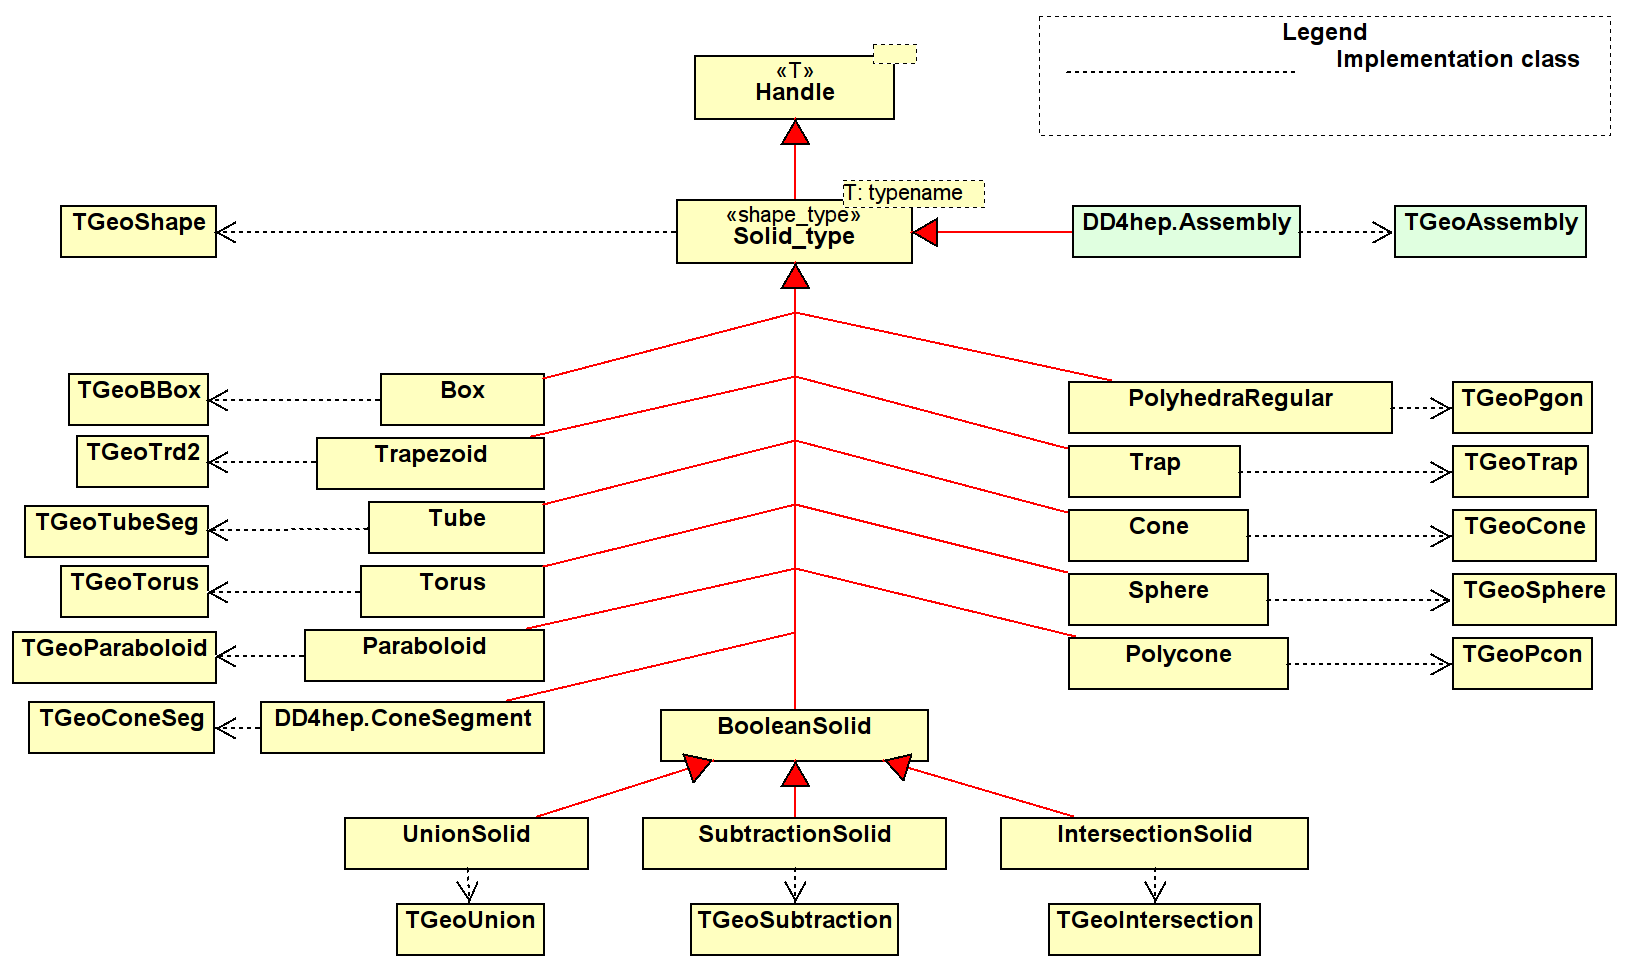
\includegraphics[width=160mm] {DD4hep-solids}
    \caption{Extensions may be attached to common Detector Elements which 
             extend the functionality of the common DetElement 
             class and support e.g. caching of precomputed values.}
    \label{fig:dd4hep-solids}
  \end{center}
  \vspace{-0.6cm}
\end{figure}

\section{Shapes}
\label{dd4hep-basic-shapes}

Shapes are abstract objects with a bounding surface and fixed dimensions.  There are primitive, atomic shapes and complex boolean shapes as shown in Figure~\ref{fig:dd4hep-solids}. The shapes have accessors for the most basic quantities to allow intrinsic access to the geometrical properties. Not all properties offered by TGeo are exposed. Other properties of the corresponding TGeo object can be accessed using the overloaded \texttt{operator->()} of the handle object. TGeo and similarly Geant4 offer a whole palette of primitive shapes, which can be used to construct more complex shapes:
\begin{itemize}
\item \texttt{Box} shape represented by the \texttt{TGeoBBox} class. To create a new box object call one of the following constructors:
\begin{minted}[frame=single,framesep=3pt,breaklines=true,tabsize=2,linenos,fontsize=\small]{c++}
/// Constructor to be used when creating an anonymous new box object
Box(double x, double y, double z);
/// Constructor to be used when creating an anonymous new box object
template<typename X, typename Y, typename Z> Box(const X& x, const Y& y, const Z& z);

/// Access half "length" of the box
double x() const;
/// Access half "width" of the box
double y() const;
/// Access half "depth" of the box
double z() const;
\end{minted}
\item \texttt{Sphere} shape represented by the \texttt{TGeoSphere} class. To create a new sphere object call one of the following constructors:
\begin{minted}[frame=single,framesep=3pt,breaklines=true,tabsize=2,linenos,fontsize=\small]{c++}
/// Constructor to create a new anonymous object with attribute initialization
Sphere(double rmin,            double rmax,
       double startTheta= 0.0, double endTheta = M_PI,
       double startPhi  = 0.0, double endPhi   = 2. * M_PI);
/// Constructor to create a new identified object with attribute initialization
Sphere(const std::string& nam, double rmin,            double rmax,
       double startTheta= 0.0, double endTheta = M_PI,
       double startPhi  = 0.0, double endPhi   = 2. * M_PI);

/// Accessor: start-phi value
double startPhi() const;
/// Accessor: end-phi value 
double endPhi() const;
/// Accessor: start-theta value
double startTheta() const;
/// Accessor: end-theta value
double endTheta() const;
/// Accessor: r-min value
double rMin() const;
/// Accessor: r-max value
double rMax() const;
\end{minted}

\item \texttt{Cone}  shape represented by the \texttt{TGeoCone} class. To create a new cone object call one of the following constructors:
\begin{minted}[frame=single,framesep=3pt,breaklines=true,tabsize=2,linenos,fontsize=\small]{c++}
/// Constructor to create a new anonymous object with attribute initialization
Cone(double z,double rmin1,double rmax1,double rmin2,double rmax2);
template<typename Z, typename RMIN1, typename RMAX1, typename RMIN2, typename RMAX2>
Cone(const Z& z, const RMIN1& rmin1, const RMAX1& rmax1, const RMIN2& rmin2, const RMAX2& rmax2);

/// Accessor: delta-z value
double dZ() const;
/// Accessor: r-min-1 value
double rMin1() const;
/// Accessor: r-min-2 value
double rMin2() const;
/// Accessor: r-max-1 value
double rMax1() const;
/// Accessor: r-max-2 value
double rMax2() const;
\end{minted}

\item \texttt{ConeSegment} shape represented by the \texttt{TGeoConeSeg} class. To create a new cone segment object call one of the following constructors:
\begin{minted}[frame=single,framesep=3pt,breaklines=true,tabsize=2,linenos,fontsize=\small]{c++}
/// Constructor to create a new ConeSegment
ConeSegment(double dz, double rmin1, double rmax1, double rmin2, double rmax2, double phi1=0.0, double phi2=2.0*M_PI);
/// Constructor to create a new named ConeSegment object
ConeSegment(const std::string& nam, double dz, double rmin1, double rmax1,
            double rmin2, double rmax2, double startPhi = 0.0, double endPhi = 2.0 * M_PI);

/// Accessor: start-phi value
double startPhi() const;
/// Accessor: end-phi value
double endPhi() const;
/// Accessor: delta-z value
double dZ() const;
/// Accessor: r-min-1 value
double rMin1() const;
/// Accessor: r-min-2 value
double rMin2() const;
/// Accessor: r-max-1 value
double rMax1() const;
/// Accessor: r-max-2 value
double rMax2() const;
\end{minted}

\item \texttt{Polycone} shape represented by the \texttt{TGeoPcon} class. To create a new polycone object call one of the following constructors:
\begin{minted}[frame=single,framesep=3pt,breaklines=true,tabsize=2,linenos,fontsize=\small]{c++}
/// Constructor to create a new polycone object
Polycone(double start, double delta);
followed by a call to:
void addZPlanes(const std::vector<double>& rmin, 
                const std::vector<double>& rmax,
                const std::vector<double>& z);
/// Constructor to create a new polycone object. Add at the same time all Z planes
Polycone(double start, double delta, 
         const std::vector<double>& rmin, 
         const std::vector<double>& rmax, 
         const std::vector<double>& z);
         
/// Accessor: start-phi value
double startPhi() const;
/// Accessor: delta-phi value
double deltaPhi() const;
/// Accessor: z value
double z(int which) const;
/// Accessor: r-min value  
double rMin(int which) const;
/// Accessor: r-max value
double rMax(int which) const;
/// Accessor: vector of z-values for Z-planes value
std::vector<double> zPlaneZ() const;
/// Accessor: vector of rMin-values for Z-planes value
std::vector<double> zPlaneRmin() const;
/// Accessor: vector of rMax-values for Z-planes value
std::vector<double> zPlaneRmax() const;
\end{minted}

\item \texttt{TubeSegment} shape represented by the \tgeo{TGeoTubeSeg}{\texttt TGeoTubeSeg} class. To create a new tube segment object call one of the following constructors:
\begin{minted}[frame=single,framesep=3pt,breaklines=true,tabsize=2,linenos,fontsize=\small]{c++}
Tube(double rmin, double rmax, double z, double deltaPhi=2*M_PI)
Tube(double rmin, double rmax, double z, double startPhi, double deltaPhi)

template<typename RMIN, typename RMAX, typename Z, typename DELTAPHI>
Tube(const RMIN& rmin, const RMAX& rmax, const Z& z, const DELTAPHI& deltaPhi)  

template<typename RMIN, typename RMAX, typename Z, typename STARTPHI, typename DELTAPHI>
Tube(const std::string& name, const RMIN& rmin, const RMAX& rmax, const Z& z, 
     const STARTPHI& startPhi, const DELTAPHI& deltaPhi)  

/// Accessor: start-phi value
double startPhi() const;
/// Accessor: end-phi value
double endPhi() const;
/// Accessor: delta-z value
double dZ() const;
/// Accessor: r-min value
double rMin() const;
/// Accessor: r-max value
double rMax() const;
\end{minted}

\item \texttt{CutTube} shape represented by the \tgeo{TGeoCtub}{\texttt TGeoCtub} class.
To create a new cut tube segment object call one of the following constructors:
\begin{minted}[frame=single,framesep=3pt,breaklines=true,tabsize=2,linenos,fontsize=\small]{c++}
/// Constructor to create a new cut-tube object with attribute initialization
CutTube(double rmin, double rmax, double dz, double startPhi, double endPhi,
        double lx, double ly, double lz, double tx, double ty, double tz);
/// Constructor to create a new identifiable cut-tube object with attribute initialization
CutTube(const std::string& name,
        double rmin, double rmax, double dz, double startPhi, double endPhi,
        double lx, double ly, double lz, double tx, double ty, double tz);

/// Accessor: start-phi value
double startPhi() const;
/// Accessor: end-phi value
double endPhi() const;
/// Accessor: delta-z value
double dZ() const;
/// Accessor: r-min value
double rMin() const;
/// Accessor: r-max value
double rMax() const;
/// Accessor: lower normal vector of cut plane
std::vector<double> lowNormal()  const;
/// Accessor: upper normal vector of cut plane
std::vector<double> highNormal() const;
\end{minted}

\item \texttt{EllipticalTube} shape represented by the \tgeo{TGeoEltu}{\texttt TGeoEltu} class.
To create a new elliptical tube segment object call one of the following constructors:
\begin{minted}[frame=single,framesep=3pt,breaklines=true,tabsize=2,linenos,fontsize=\small]{c++}
/// Constructor to create a new anonymous tube object with attribute initialization
EllipticalTube(double a, double b, double dz);
/// Constructor to create a new identified tube object with attribute initialization
EllipticalTube(const std::string& nam, double a, double b, double dz);

/// Accessor: delta-z value
double dZ() const;
/// Accessor: a value (semi axis along x)
double a() const;
/// Accessor: b value (semi axis along y)
double b() const;
\end{minted}

\item \texttt{Trapezoid} shape represented by the \texttt{TGeoTrd2} class. To create a new trapezoid object call one of the following constructors:
\begin{minted}[frame=single,framesep=3pt,breaklines=true,tabsize=2,linenos,fontsize=\small]{c++}
/// Constructor to create a new anonymous object with attribute initialization
Trapezoid(double x1, double x2, double y1, double y2, double z);
/// Constructor to create a new anonymous object with attribute initialization
template <typename X1,typename X2,typename Y1,typename Y2,typename Z>
Trd2(X1 x1, X2 x2, Y1 y1, Y2 y2, Z z);
/// Constructor to create a new identified object with attribute initialization
Trd2(const std::string& nam, double x1, double x2, double y1, double y2, double z);
/// Constructor to create a new identified object with attribute initialization
template <typename X1,typename X2,typename Y1,typename Y2,typename Z>
Trd2(const std::string& nam, X1 x1, X2 x2, Y1 y1, Y2 y2, Z z);

/// Accessor: delta-x1 value
double dX1() const;
/// Accessor: delta-x2 value
double dX2() const;
/// Accessor: delta-y1 value
double dY1() const;
/// Accessor: delta-y2 value
double dY2() const;
/// Accessor: delta-z value
double dZ() const;
\end{minted}

\item \texttt{Trap} shape represented by the \tgeo{TGeoTrap}{\texttt TGeoTrap} class. To create a new trap object call one of the following constructors:
\begin{minted}[frame=single,framesep=3pt,breaklines=true,tabsize=2,linenos,fontsize=\small]{c++}
/// Constructor to create a new anonymous object with attribute initialization
Trap(double z,double theta,double phi,
     double y1,double x1,double x2,double alpha1,
     double y2,double x3,double x4,double alpha2);
/// Constructor to create a new anonymous object for right angular wedge from STEP (Se G4 manual for details)
Trap( double pz, double py, double px, double pLTX);

/// Accessor: phi value
double phi() const;
/// Accessor: theta value
double theta() const;
/// Angle between centers of x edges and y axis at low z
double alpha1()  const;
/// Angle between centers of x edges and y axis at low z
double alpha2()  const;
/// Half length in x at low z and y low edge
double bottomLow1()  const;
/// Half length in x at high z and y low edge
double bottomLow2()  const;
/// Half length in x at low z and y high edge
double topLow1()  const;
/// Half length in x at high z and y high edge
double topLow2()  const;
/// Half length in y at low z
double high1()  const;
/// Half length in y at high z
double high2()  const;
/// Half length in dZ
double dZ()  const;
\end{minted}

\item \texttt{Torus}  shape represented by the \tgeo{TGeoTorus}{\texttt TGeoTorus} class. To create a new torus object call one of the following constructors:
\begin{minted}[frame=single,framesep=3pt,breaklines=true,tabsize=2,linenos,fontsize=\small]{c++}
/// Constructor to create a new anonymous object with attribute initialization
Torus(double r, double rmin, double rmax, double phi=M_PI, double delta_phi=2.*M_PI);

/// Accessor: start-phi value
double startPhi() const;
/// Accessor: delta-phi value
double deltaPhi() const;

/// Accessor: r value (torus axial radius)
double r() const;
/// Accessor: r-min value (inner radius)
double rMin() const;
/// Accessor: r-max value (outer radius)
double rMax() const;
\end{minted}

\item \texttt{Paraboloid}  shape represented by the \tgeo{TGeoParaboloid}{\texttt TGeoParaboloid} class. To create a new paraboloid object call one of the following constructors:
\begin{minted}[frame=single,framesep=3pt,breaklines=true,tabsize=2,linenos,fontsize=\small]{c++}
/// Constructor to create a new anonymous object with attribute initialization
Paraboloid(double r_low, double r_high, double delta_z);

/// Accessor: delta-z value
double dZ() const;
/// Accessor: r-min value
double rLow() const;
/// Accessor: r-max value
double rHigh() const;
\end{minted}

\item \texttt{Hyperboloid}  shape represented by the \tgeo{TGeoHype}{\texttt TGeoHype} class. To create a new hyperboloid object call one of the following constructors:
\begin{minted}[frame=single,framesep=3pt,breaklines=true,tabsize=2,linenos,fontsize=\small]{c++}
/// Constructor to create a new anonymous object with attribute initialization
Hyperboloid(double rin, double stin, double rout, double stout, double dz);
/// Constructor to create a new identified object with attribute initialization
Hyperboloid(const std::string& nam, double rin, double stin, double rout, double stout, double dz);

/// Accessor: delta-z value
double dZ() const;
/// Accessor: r-min value
double rMin() const;
/// Accessor: r-max value
double rMax() const;
/// Stereo angle for inner surface
double stereoInner()  const;
/// Stereo angle for outer surface
double stereoOuter()  const;
\end{minted}

\item \texttt{PolyhedraRegular} shape represented by the \texttt{TGeoPgon} class. To create a new polyhedron object call one of the following constructors:
\begin{minted}[frame=single,framesep=3pt,breaklines=true,tabsize=2,linenos,fontsize=\small]{c++}
/// Constructor to create a new object. Phi(start)=0, deltaPhi=2PI, Z-planes at +-zlen/2
PolyhedraRegular(int nsides, double rmin, double rmax, double zlen);
/// Constructor to create a new object. Phi(start)=0, deltaPhi=2PI, Z-planes at zplanes[0],[1]
PolyhedraRegular(int nsides, double rmin, double rmax, double zplanes[2]);
/// Constructor to create a new object with phi_start, deltaPhi=2PI, Z-planes at +-zlen/2
PolyhedraRegular(int nsides, double phi_start, double rmin, double rmax, double zlen);

/// Accessor: Number of edges
int numEdges()  const;
/// Accessor: start-phi value
double startPhi() const;
/// Accessor: delta-phi value
double deltaPhi() const;

/// Accessor: r-min value
double z(int which) const;
/// Accessor: r-min value
double rMin(int which) const;
/// Accessor: r-max value
double rMax(int which) const;

/// Accessor: vector of z-values for Z-planes value
std::vector<double> zPlaneZ() const;
/// Accessor: vector of rMin-values for Z-planes value
std::vector<double> zPlaneRmin() const;
/// Accessor: vector of rMax-values for Z-planes value
std::vector<double> zPlaneRmax() const;
\end{minted}

\item \texttt{Polyhedra} shape represented by the \texttt{TGeoPgon} class. To create a new generic polyhedron object call one of the following constructors:
\begin{minted}[frame=single,framesep=3pt,breaklines=true,tabsize=2,linenos,fontsize=\small]{c++}
/// Constructor to create a new object. Phi(start), deltaPhi, Z-planes at specified positions
Polyhedra(int nsides, double start, double delta, const std::vector<double>& z, const std::vector<double>& r);
/// Constructor to create a new object. Phi(start), deltaPhi, Z-planes at specified positions
Polyhedra(int nsides, double start, double delta,
          const std::vector<double>& z, const std::vector<double>& rmin, const std::vector<double>& rmax)

/// Accessor: Number of edges
int numEdges()  const;
/// Accessor: start-phi value
double startPhi() const;
/// Accessor: delta-phi value
double deltaPhi() const;

/// Accessor: z value
double z(int which) const;
/// Accessor: r-min value
double rMin(int which) const;
/// Accessor: r-max value
double rMax(int which) const;

/// Accessor: vector of z-values for Z-planes value
std::vector<double> zPlaneZ() const;
/// Accessor: vector of rMin-values for Z-planes value
std::vector<double> zPlaneRmin() const;
/// Accessor: vector of rMax-values for Z-planes value
std::vector<double> zPlaneRmax() const;
\end{minted}

\item \texttt{ExtrudedPolygon} shape represented by the \texttt{TGeoXtru} class. To create a new extruded polygon object call one of the following constructors:
\begin{minted}[frame=single,framesep=3pt,breaklines=true,tabsize=2,linenos,fontsize=\small]{c++}
/// Constructor to create a new object. 
ExtrudedPolygon(const std::vector<double> & pt_x,  const std::vector<double> & pt_y,
                const std::vector<double> & sec_z, const std::vector<double> & sec_x, const std::vector<double> & sec_y,
                const std::vector<double> & zscale);
/// Constructor to create a new identified object. 
ExtrudedPolygon(const std::string& nam,
                const std::vector<double> & pt_x,  const std::vector<double> & pt_y,
                const std::vector<double> & sec_z, const std::vector<double> & sec_x, const std::vector<double> & sec_y,
                const std::vector<double> & zscale);

/// Access vector of x parameters of the various vertices
std::vector<double> x() const;
/// Access vector of x parameters of the various vertices
std::vector<double> y() const;
/// Access vector of z-values of the z plane parameters
std::vector<double> z() const;
/// Access vector of x-offsets of the z plane parameters
std::vector<double> zx() const;
/// Access vector of y-offsets of the z plane parameters
std::vector<double> zy() const;
/// Access vector of z-scale parameters
std::vector<double> zscale() const;
\end{minted}

\item \texttt{EightPointSolid} shape represented by the \texttt{TGeoArb8} class. To create a generic solid defined by eight vertices call one of the following constructors:
\begin{minted}[frame=single,framesep=3pt,breaklines=true,tabsize=2,linenos,fontsize=\small]{c++}
/// Constructor to create a new anonymous object with attribute initialization
EightPointSolid(double dz, const double* vertices);
/// Constructor to create a new identified object with attribute initialization
EightPointSolid(const std::string& nam, double dz, const double* vertices);

/// Accessor: delta-z value
double dZ() const;
/// Accessor: all vertices as STL vector
std::vector<double> vertices() const;
/// Accessor: single vertex
std::pair<double, double> vertex(int which) const;
\end{minted}

\item \texttt{TessellatedSolid} shape represented by the \texttt{TGeoTessellated} class. To create a generic solid defined by eight vertices call one of the following constructors:
\begin{minted}[frame=single,framesep=3pt,breaklines=true,tabsize=2,linenos,fontsize=\small]{c++}
/// Constructor to create a new anonymous object with attribute initialization
TessellatedSolid(int num_facets);
/// Constructor to create a new identified object with attribute initialization
TessellatedSolid(const std::vector<Vertex_t>& vertices);
/// Constructor to create a new anonymous object with attribute initialization
TessellatedSolid(const std::string& nam, int num_facets);
/// Constructor to create a new identified object with attribute initialization
TessellatedSolid(const std::string& nam, const std::vector<Vertex_t>& vertices);

/// Add new facet to the shape
bool addFacet(const Vertex_t& pt0, const Vertex_t& pt1, const Vertex_t& pt2)  const;
/// Add new facet to the shape
bool addFacet(const Vertex_t& pt0, const Vertex_t& pt1, const Vertex_t& pt2, const Vertex_t& pt3)  const;
/// Add new facet to the shape. Call only if the tessellated shape was constructed with vertices
bool addFacet(const int pt0, const int pt1, const int pt2)  const;
/// Add new facet to the shape. Call only if the tessellated shape was constructed with vertices
bool addFacet(const int pt0, const int pt1, const int pt2, const int pt3)  const;
\end{minted}
Tessellated shapes play an essential role to support reading Computer Aided Design files in DD4hep. Such support is implemented in the DD4hep subpackage \texttt{DDCAD}.

\end{itemize}

Besides the primitive shapes three types of boolean shapes (described in TGeo by the \texttt{TGeoCompositeShape} class) are supported:

\begin{itemize}
\item \texttt{UnionSolid} objects representing the union,
\item \texttt{IntersectionSolid} objects representing the intersection,
\item \texttt{SubtractionSolid} objects representing the subtraction,
\end{itemize}

of two other primitive or complex shapes. To build a boolean shape, the second shape is transformed in 3-dimensional space before the boolean operation is applied. The 3D transformations are described by objects from the \texttt{ROOT::Math} library and are supplied at construction time.  Such a transformation as shown in the code snippet below may be 

\begin{itemize}
\item The identity transformation. Then no transformation object needs to be provided (see line 2).
\item A translation only described by a \texttt{Position} object (see line 4)
\item A 3-fold rotation first around the Z-axis, then around the Y-axis and finally around the X-axis. For transformation operations of this kind a \texttt{RotationZYX} object must be supplied (see line 6).
\item A generic 3D rotation matrix should be applied to the second shape. Then a \texttt{Rotation3D} object must be supplied (see line 8).
\item Finally a generic 3D transformation (translation+rotation) may be applied using a \texttt{Transform3D} object (see line 10).
\end{itemize}

All three boolean shapes have constructors as shown here for the \texttt{UnionSolid}:
\begin{minted}[frame=single,framesep=3pt,breaklines=true,tabsize=2,linenos,fontsize=\small]{c++}
  /// Constructor to create a new object. Position is identity, Rotation is identity-rotation!
  UnionSolid(const Solid& shape1, const Solid& shape2);
  /// Constructor to create a new object. Placement by position, Rotation is identity-rotation!
  UnionSolid(const Solid& shape1, const Solid& shape2, const Position& pos);
  /// Constructor to create a new object. Placement by a RotationZYX within the mother
  UnionSolid(const Solid& shape1, const Solid& shape2, const RotationZYX& rot);
  /// Constructor to create a new object. Placement by a generic rotation within the mother
  UnionSolid(const Solid& shape1, const Solid& shape2, const Rotation3D& rot);
  /// Constructor to create a new object. Placement by a generic transformation within the mother
  UnionSolid(const Solid& shape1, const Solid& shape2, const Transform3D& pos);
\end{minted}
\newpage

\subsection{Shape factories} 
Sometimes it is useful to create shapes in an ``abstract'' way e.g. to define areas in the detector. To create such shapes a factory method was implemented, which allows to create a valid shape handle given a valid \texttt{XML} element providing the required attributes. The factory methods are invoked using from \texttt{XML} elements of the following form:
\begin{minted}[frame=single,framesep=3pt,breaklines=true,tabsize=2,linenos,fontsize=\small]{xml}
  <some_element type="shape-type" .... args ....>
\end{minted}

The shape is then constructed using the \texttt{XML} component object:
\begin{minted}[frame=single,framesep=3pt,breaklines=true,tabsize=2,linenos,fontsize=\small]{c++}
#include "XML/Helper.h"

xml_h e = <shape-element>;
Box box = xml_comp_t(e).createShape();
if ( !box.isValid() ) { /* ...handle error ... */  }
\end{minted}
The required arguments for the various shapes are then:
\begin{itemize}
\item For a Box:
\begin{minted}[frame=single,framesep=3pt,breaklines=true,tabsize=2,linenos,fontsize=\small]{xml}
  <some_element type="Box" x="x-value" y="y-value" z="z-value"/>
\end{minted}
fulfilling a constructor of the type: \texttt{Box(dim.dx(), dim.dy(), dim.dz())}.

\item For a Sphere the following constructor must be fulfilled: 
\begin{minted}[frame=single,framesep=3pt,breaklines=true,tabsize=2,linenos,fontsize=\small]{c++}
  Sphere(e.rmin(0), e.rmax(), e.starttheta(0), e.endtheta(), e.startphi(0), e.endphi());
\end{minted}
The corresponding XML snippet looks like this:
\begin{minted}[frame=single,framesep=3pt,breaklines=true,tabsize=2,linenos,fontsize=\small]{c++}
  <some_element type="Sphere" rmin="value" rmax="value" starttheta="value" endtheta="value" startphi="value" endphi="value"/>
\end{minted}
where the above default values for the \texttt{XML} attributes \texttt{rmin=0}, \texttt{starttheta=0}, \texttt{endtheta=$\pi$},
\texttt{startphi=0}, \texttt{endphi=$2\times\pi$}.

\item For a Cone the following constructor must be fulfilled: 
\begin{minted}[frame=single,framesep=3pt,breaklines=true,tabsize=2,linenos,fontsize=\small]{c++}
  double rmi1 = e.rmin1(0), rma1 = e.rmax1();
  Cone(e.z(0), rmi1, rma1, e.rmin2(rmi1), e.rmax2(rma1));
\end{minted}
The corrsponding XML snippet looks like this:
\begin{minted}[frame=single,framesep=3pt,breaklines=true,tabsize=2,linenos,fontsize=\small]{xml}
  <some_element type="Cone" z="value" rmin1="value" rmax1="value" rmin2="value" rmax2="value"/>
\end{minted}
where the above default values for the \texttt{XML} attributes \texttt{rmin1=0}, \texttt{rmin2=rmin1}, \texttt{rmax2=rmax1}.

\item For a ConeSegment the following constructor must be fulfilled: 
\begin{minted}[frame=single,framesep=3pt,breaklines=true,tabsize=2,linenos,fontsize=\small]{c++}
ConeSegment(e.dz(), e.rmin1(0), e.rmax1(), e.rmin2(), e.rmax2(), e.startphi(), e.deltaphi())
\end{minted}
where the above default values for the \texttt{XML} attributes \texttt{rmin1=0}, \texttt{rmin2=0},
\texttt{rmax2=rmax1}, \texttt{startphi=0} and \texttt{deltaphi=$2\times\pi$}
are used if not explicitly stated in the \texttt{XML} element \texttt{e}.
The corrsponding XML snippet looks like this:
\begin{minted}[frame=single,framesep=3pt,breaklines=true,tabsize=2,linenos,fontsize=\small]{xml}
  <some_element type="ConeSegment" rmin1="value" rmax="value" rmin2="value" rmax2="value" dz="value" startphi="value" deltaphi="value"/>
\end{minted}

\item For a Polycone:
\vspace{-0.2cm}
\begin{minted}[frame=single,framesep=3pt,breaklines=true,tabsize=2,linenos,fontsize=\small]{xml}
  <some_element type="Polycone" start="start-phi-value" deltaphi="delta-phi-value">
    <zplane z="z-value" rmin="rmin-value" rmax="rmax-value"/>
    <zplane z="z-value" rmin="rmin-value" rmax="rmax-value"/>
    .... any number of Z-planes ....
    <zplane z="z-value" rmin="rmin-value" rmax="rmax-value"/>
  </some_element>
\end{minted}
where the above default values for the \texttt{XML} attributes \texttt{startphi=0} and
\texttt{deltaphi=$2\times\pi$} and for each of the the z-planes \texttt{rmin=0}
are used if not explicitly stated in the \texttt{XML} element \texttt{e}.

\item For a Tube the constructor is:
\begin{minted}[frame=single,framesep=3pt,breaklines=true,tabsize=2,linenos,fontsize=\small]{c++}
Tube(e.rmin(0.0), e.rmax(), e.dz(), e.startphi(), e.deltaphi())
\end{minted}
The corrsponding XML snippet looks like this:
\begin{minted}[frame=single,framesep=3pt,breaklines=true,tabsize=2,linenos,fontsize=\small]{xml}
  <some_element type="Tube" rmin="value" rmax="value" dz="value" startphi="value" deltaphi="value"/>
\end{minted}
where the defaults are \texttt{rmin=0}, \texttt{startphi=0} and \texttt{deltaphi=$2\times\pi$}.

\item For a CutTube the constructor is:
\begin{minted}[frame=single,framesep=3pt,breaklines=true,tabsize=2,linenos,fontsize=\small]{c++}
CutTube(e.rmin(0.0), e.rmax(), e.dz(), e.phi1(), e.phi2(), e.lx(), e.ly(), e.lz(), e.tx(), e.ty(), e.tz())
\end{minted}
The corrsponding XML snippet looks like this:
\begin{minted}[frame=single,framesep=3pt,breaklines=true,tabsize=2,linenos,fontsize=\small]{xml}
  <some_element type="CutTube" rmin="value" rmax="value" dz="value" phi1="value" phi2="value"
                lx="value" ly="value" lz="value" tx="value" ty="value" tz="value"/>
\end{minted}
where the defaults are \texttt{rmin=0}.

\item For a EllipticalTube the constructor is:
\begin{minted}[frame=single,framesep=3pt,breaklines=true,tabsize=2,linenos,fontsize=\small]{c++}
EllipticalTube(e.a(),e.b(),e.dz());
\end{minted}
The corrsponding XML snippet looks like this:
\begin{minted}[frame=single,framesep=3pt,breaklines=true,tabsize=2,linenos,fontsize=\small]{xml}
  <some_element type="EllipticalTube" dz="value" a="value" b="value"/>
\end{minted}

\item For a Trap the constructor is: if \texttt{dz} is specified: 
\begin{minted}[frame=single,framesep=3pt,breaklines=true,tabsize=2,linenos,fontsize=\small]{c++}
Trap(e.dz(), e.dy(), e.dx(),_toDouble(_Unicode(pLTX)))
\end{minted}
Alternatively, if the tag  \texttt{dz} is not present: 
\begin{minted}[frame=single,framesep=3pt,breaklines=true,tabsize=2,linenos,fontsize=\small]{c++}
Trap(e.z(0.0), e.theta(), e.phi(0), e.y1(), e.x1(), e.x2(), e.alpha1(), e.y2(), e.x3(), e.x4(), e.alpha2())
\end{minted}
The corrsponding XML snippet looks like this:
\begin{minted}[frame=single,framesep=3pt,breaklines=true,tabsize=2,linenos,fontsize=\small]{xml}
  <some_element type="Trap" z="value" theta="value" phi="value"
                            y1="value" x1="value" x2="value" alpha1="value"
                            y2="value" x3="value" x4="value" alpha2="value"/>
\end{minted}
Defaults are: \texttt{theta=0},  \texttt{phi=0},  \texttt{alpha1=0},  \texttt{alpha2=0}

\item For a Trapezoid the constructor is:
\begin{minted}[frame=single,framesep=3pt,breaklines=true,tabsize=2,linenos,fontsize=\small]{c++}
Trapezoid(e.x1(), e.x2(), e.y(), e.z(0))
\end{minted}
The corrsponding XML snippet looks like this:
\begin{minted}[frame=single,framesep=3pt,breaklines=true,tabsize=2,linenos,fontsize=\small]{xml}
  <some_element type="Trapezoid" x1="value" x2="value" y="value" z="value"/>
\end{minted}
The Trapezoid is also aliased to Trd2.

\item For a simplified Trapezoid, the Trd1 the constructor is:
\begin{minted}[frame=single,framesep=3pt,breaklines=true,tabsize=2,linenos,fontsize=\small]{c++}
Trd1(e.x1(), e.x2(), e.y1(), e.y2(), e.z(0));
\end{minted}
The corrsponding XML snippet looks like this:
\begin{minted}[frame=single,framesep=3pt,breaklines=true,tabsize=2,linenos,fontsize=\small]{xml}
  <some_element type="Trd1" x1="value" x2="value" y1="value" y2="value" z="value"/>
\end{minted}

\item For a Torus the constructor is:
\begin{minted}[frame=single,framesep=3pt,breaklines=true,tabsize=2,linenos,fontsize=\small]{c++}
Torus(e.r(), e.rmin(), e.rmax(), e.startphi(), e.deltaphi())
\end{minted}
The corrsponding XML snippet looks like this:
\begin{minted}[frame=single,framesep=3pt,breaklines=true,tabsize=2,linenos,fontsize=\small]{xml}
  <some_element type="Torus" r="value" rmin="value" rmax="value" startphi="value" deltaphi="value"/>
\end{minted}
Defaults are: \texttt{rmin=0},  \texttt{startphi=$\pi$},  \texttt{deltaphi=$2\times\pi$}.

\item For a Sphere the constructor is:
\begin{minted}[frame=single,framesep=3pt,breaklines=true,tabsize=2,linenos,fontsize=\small]{c++}
Sphere(e.rmin(), e.rmax(), e.starttheta(), e.deltatheta(), e.startphi(), e.deltaphi())
\end{minted}
The corrsponding XML snippet looks like this:
\begin{minted}[frame=single,framesep=3pt,breaklines=true,tabsize=2,linenos,fontsize=\small]{xml}
  <some_element type="Sphere" rmin="value" rmax="value"
                starttheta="value" deltatheta="value" startphi="value" deltaphi="value"/>
\end{minted}
Defaults are: \texttt{rmin=0},  \texttt{starttheta=0},  \texttt{deltatheta=$\pi$},
\texttt{startphi=0}, \texttt{deltaphi=$2\times\pi$}.

\item For a Paraboloid the constructor is:
\begin{minted}[frame=single,framesep=3pt,breaklines=true,tabsize=2,linenos,fontsize=\small]{c++}
Paraboloid(e.rmin(0), e.rmax(), e.dz())
\end{minted}
The corrsponding XML snippet looks like this:
\begin{minted}[frame=single,framesep=3pt,breaklines=true,tabsize=2,linenos,fontsize=\small]{xml}
  <some_element type="Paraboloid" rmin="value" rmax="value" dz="value"/>
\end{minted}
Defaults are: \texttt{rmin=0}.

\item For a Hyperboloid the constructor is:
\begin{minted}[frame=single,framesep=3pt,breaklines=true,tabsize=2,linenos,fontsize=\small]{c++}
Hyperboloid(e.rmin(0), e.inner_stereo(), e.rmax(), e.outer_stereo, e.dz())
\end{minted}
The corrsponding XML snippet looks like this:
\begin{minted}[frame=single,framesep=3pt,breaklines=true,tabsize=2,linenos,fontsize=\small]{xml}
  <some_element type="Hyperboloid" rmin="value" inner_stereo="value" rmax="value" outer_stereo=="value" dz="value"/>
\end{minted}

\item For a PolyhedraRegular the constructor is:
\begin{minted}[frame=single,framesep=3pt,breaklines=true,tabsize=2,linenos,fontsize=\small]{c++}
PolyhedraRegular(e.numsides(), e.rmin(), e.rmax(), e.dz())
\end{minted}
The corrsponding XML snippet looks like this:
\begin{minted}[frame=single,framesep=3pt,breaklines=true,tabsize=2,linenos,fontsize=\small]{xml}
  <some_element type="PolyhedraRegular" numsides="value" rmin="value" rmax="value" dz="value"/>
\end{minted}

\item For a generic Polyhedra the constructor is:
\begin{minted}[frame=single,framesep=3pt,breaklines=true,tabsize=2,linenos,fontsize=\small]{c++}
PolyhedraRegular(e.numsides(), e.rmin(), e.startphi(), e.deltaphi(), vector<z>, vector<rmin>, vector<rmax>);
\end{minted}
The corrsponding XML snippet looks like this:
\begin{minted}[frame=single,framesep=3pt,breaklines=true,tabsize=2,linenos,fontsize=\small]{xml}
  <some_element type="Polyhedra" numsides="value" startphi="value" deltaphi="value">
    <plane z="z-value" rmin="rmin-value" rmax="rmax-value"/>
    <plane z="z-value" rmin="rmin-value" rmax="rmax-value"/>
    ...
  <some_element/>
\end{minted}

\item For a generic eight point solid the constructor is:
\begin{minted}[frame=single,framesep=3pt,breaklines=true,tabsize=2,linenos,fontsize=\small]{c++}
EightPointSolid(e.dz(), vertices);
\end{minted}
The corrsponding XML snippet looks like this:
\begin{minted}[frame=single,framesep=3pt,breaklines=true,tabsize=2,linenos,fontsize=\small]{xml}
  <some_element type="EightPointSolid" dz="value">
    <vertex x="x-value" y="y-value"/>
    <vertex x="x-value" y="y-value"/>
    ...exactly 8 vertices in total...
  <some_element/>
\end{minted}

\item For a boolean shape the xml snippet is nested and contains 2 shape descriptions:
\begin{minted}[frame=single,framesep=3pt,breaklines=true,tabsize=2,linenos,fontsize=\small]{xml}
  <some_element type="BooleanShape" operation="value">
    <shape ....description of left hand shape/>
    <shape ....description of right hand shape/>

    <transformation  ...generic transformation description.../>
    <!-- OR  -->
    <position x="value" y="value" z="value"/>
    <rotation x="value" y="value" z="value"/>
  <some_element/>
\end{minted}
valid operations are \texttt{subtraction}, \texttt{union} and \texttt{intersection}.

\end{itemize}

\section{Volumes and Placements}

The detector geometry is described by a hierarchy of volumes and their  corresponding placements. Both, the TGeo package and Geant4~\cite{Agostinelli:2002hh} are following effectively the same ideas ensuring an easy conversion from TGeo to Geant4 objects for the simulation application. A volume is an unplaced solid de\-scribed in terms of a primitive shape or a boolean operation of solids, a material and a number of placed sub-volumes (placed volumes) inside. The class diagram showing the relationships between volumes and placements, solids and materials is shown in Figure~\ref{fig:dd4hep-detector-model}.
It is worth noting, that any volume has children, but no parent or ``mother'' volume. This is a direct consequence of the requirement to re-use volumes and place the same volume arbitrarily often. Only the act of placing a volume defines the relationship to the next level parent volume. The resulting geometry tree is very effective, simple and convenient to  describe the detector geometry hierarchy starting from the top level volume representing e.g. the experiment cavern down to the very detail of the detector e.g. the small screw in the calorimeter. The top level volume is the very only volume without a placement. All geometry calculations, computations are always  performed within the local coordinate system of the volume. The following example code shows how to create a volume which consists of a given material and with a shape. The created volume is then placed inside the mother-volume using the local coordinate system of the mother volume:

\begin{minted}[frame=single,framesep=3pt,breaklines=true,tabsize=2,linenos,fontsize=\small]{c++}
  Volume       mother = ....ampercent

  Material     mat    (lcdd.material("Iron"));
  Tube         tub    (rmin, rmax, zhalf);
  Volume       vol    (name, tub, mat);
  Transform3D  tr     (RotationZYX(rotz,roty,rotx),Position(x,y,z));
  PlacedVolume phv = mother.placeVolume(vol,tr);
\end{minted}

The volume has the shape of a tube and consists of iron. Before being placed, the daughter volume is transformed within the mother coordinate system according to the requested transformation. The example also illustrates how to access \texttt{Material} objects from the \texttt{Detector} interface.

The {\texttt{Volume}} class provides several possibilities to declare the required space transformation necessary to place a daughter volume  within the mother:
\begin{itemize}
\item to place a daughter volume unrotated at the origin of the mother, the 
transformation is the identity. Use the following call to place the daughter:
\begin{minted}[frame=single,framesep=3pt,breaklines=true,tabsize=2,linenos,fontsize=\small]{c++}
PlacedVolume placeVolume(const Volume& vol)  const;
\end{minted}
\item If the positioning is described by a simple translation, use:
\begin{minted}[frame=single,framesep=3pt,breaklines=true,tabsize=2,linenos,fontsize=\small]{c++}
PlacedVolume placeVolume(const Volume& vol, const Position& pos)  const;
\end{minted}
\item In case the daughter should be rotated first around the Z-axis, then around the Y-axis and finally around the X-axis place the daughter using this call:
\begin{minted}[frame=single,framesep=3pt,breaklines=true,tabsize=2,linenos,fontsize=\small]{c++}
PlacedVolume placeVolume(const Volume& vol, const RotationZYX& rot)  const;
\end{minted}
\item If the full 3-dimensional rotation matrix is known use:
\begin{minted}[frame=single,framesep=3pt,breaklines=true,tabsize=2,linenos,fontsize=\small]{c++}
PlacedVolume placeVolume(const Volume& vol, const Rotation3D& rot)  const;
\end{minted}
\item for an entirely unconstrained placement place the daughter providing a \texttt{Transform3D} object:
\begin{minted}[frame=single,framesep=3pt,breaklines=true,tabsize=2,linenos,fontsize=\small]{c++}
PlacedVolume placeVolume(const Volume& volume, const Transform3D& tr)  const;
\end{minted}
\end{itemize}

For more details of the \texttt{Volume} and the \texttt{PlacedVolume} classes please see the header file \texttt{Volumes.h}.

One volume like construct is special: the assembly constructs. Assemblies are volumes without shapes. The ``assembly'' shape does not own a own surface by itself, but rather defines its surface and
bounding box from the contained children. In this corner also the implementation concepts between TGeo and Geant4 diverge. Whereas TGeo handles assemblies very similar to real volumes, in Geant4 assemblies are purely artificial and disappear at the very moment volumes  are placed.

\section{Detector Elements}
\label{sec:dd4hep-user-manual-detector-elements}

\begin{figure}[b]
  \begin{center}
    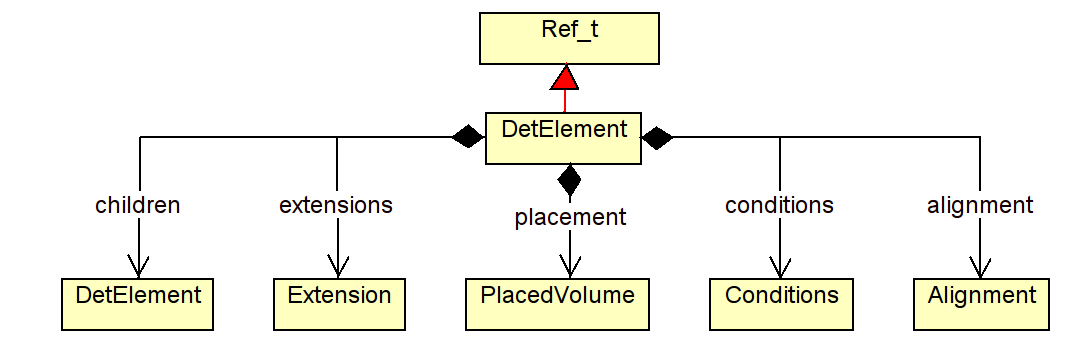
\includegraphics[width=160mm] {DD4hep-detelement-drawing}
    \caption{The basic layout of the \texttt{DetElement} class aggregating
        all data entities necessary to process data.}
    \label{fig:dd4hep-user-manual-detelement-drawing}
  \end{center}
  \vspace{-0.6cm}
\end{figure}

Detector elements (class \texttt{DetElement}) are entities which represent  subdetectors or sizable parts of a subdetector. As shown in Figure~\ref{fig:dd4hep-user-manual-detelement-drawing}, a \texttt{DetElement} instance has the means to provide to clients information about

\begin{itemize}
\item generic properties like the detector type or the path within the \texttt{DetElement}s hierarchy:
\begin{minted}[frame=single,framesep=3pt,breaklines=true,tabsize=2,linenos,fontsize=\small]{c++}
  /// Access detector type (structure, tracker, calorimeter, etc.).
  std::string type() const;
  /// Path of the detector element (not necessarily identical to placement path!)
  std::string path() const;
\end{minted}

\item the detector hierarchy by exposing its children. The hierarchy may be  accessed with the following API:
\begin{minted}[frame=single,framesep=3pt,breaklines=true,tabsize=2,linenos,fontsize=\small]{c++}
  /// Add new child to the detector structure
  DetElement& add(DetElement sub_element);
  /// Access to the list of children
  const Children& children() const;
  /// Access to individual children by name
  DetElement child(const std::string& name) const;
  /// Access to the detector element's parent
  DetElement parent() const;
\end{minted}

\item its placement within the overall experiment if it represents an entire subdetector or its placement with respect to its parent if the \texttt{DetElement} represents a part of a subdetector. The placement path is the fully qualified path of placed volumes  from the top level volume to the placed detector element. % and may serve as a shortcut for the eqnarrayment implementation:
\begin{minted}[frame=single,framesep=3pt,breaklines=true,tabsize=2,linenos,fontsize=\small]{c++}
  /// Access to the full path to the placed object
  std::string placementPath() const;
  /// Access to the physical volume of this detector element
  PlacedVolume placement() const;
  /// Access to the logical volume of the daughter placement
  Volume volume() const;
\end{minted}

\item information about the environmental conditions etc. (\texttt{conditions}):
\begin{minted}[frame=single,framesep=3pt,breaklines=true,tabsize=2,linenos,fontsize=\small]{c++}
  /// Access to the conditions information 
  Conditions conditions() const;
\end{minted}

%\item eqnarrayment information:
%\begin{minted}[frame=single,framesep=3pt,breaklines=true,tabsize=2,linenos,fontsize=\small]{c++}
%  /// Access to the eqnarrayment information
%  eqnarrayment eqnarrayment() const;
%\end{minted}

\item convenience information such as cached transformations to/from the top level volume, to/from the parent \texttt{DetElement} and to/from another \texttt{DetElement} in the hierarchy above:
\begin{minted}[frame=single,framesep=3pt,breaklines=true,tabsize=2,linenos,fontsize=\small]{c++}
  /// Transformation from local coordinates of the placed volume to the world system
  bool localToWorld(const Position& local, Position& global) const;
  /// Transformation from world coordinates of the local placed volume coordinates
  bool worldToLocal(const Position& global, Position& local) const;

  /// Transformation from local coordinates of the placed volume to the parent system
  bool localToParent(const Position& local, Position& parent) const;
  /// Transformation from world coordinates of the local placed volume coordinates
  bool parentToLocal(const Position& parent, Position& local) const;

  /// Transformation from local coordinates of the placed volume to arbitrary parent system set as reference
  bool localToReference(const Position& local, Position& reference) const;
  /// Transformation from world coordinates of the local placed volume coordinates
  bool referenceToLocal(const Position& reference, Position& local) const;

  /// Set detector element for reference transformations. 
  /// Will delete existing reference transformation.
  DetElement& setReference(DetElement reference);
\end{minted}

\item User extension information as described in section~\ref{sec:dd4hep-user-manual-data-extensions}:
\begin{minted}[frame=single,framesep=3pt,breaklines=true,tabsize=2,linenos,fontsize=\small]{c++}
  /// Extend the detector element with an arbitrary structure accessible by the type
  template <typename IFACE, typename CONCRETE> IFACE* addExtension(CONCRETE* c);
  /// Access extension element by the type
  template <class T> T* extension() const;
\end{minted}

\end{itemize}

\section{Sensitive Detectors}
\label{sec:dd4hep-user-manual-sensitive-detectors}

Though the concept of sensitive detectors comes from Geant4 and simulation  activities, in DD4hep the sensitive detectors are the client interface to  access the readout description (class \texttt{Readout}) with its  segmentation of sensitive elements (class \texttt{Segmentation}) and the description of hit decoders (class \texttt{IDDescriptors}). As shown in Figure~\ref{fig:dd4hep-sensitive-detectors}, these object instances are required when reconstructing data from particle collisions.

Besides the access to data necessary for reconstruction the sensitive detector also hosts Region setting (class \texttt{Region} and sets of cut limits (class \texttt{LimitSets}) used to configure the Geant4 simulation toolkit. The following code snippet shows the accessors of the  \texttt{SensitiveDetector} class to obtain the corresponding  information~\footnote{The methods to set the data are not shown here.}:

\begin{minted}[frame=single,framesep=3pt,breaklines=true,tabsize=2,linenos,fontsize=\small]{c++}
    struct SensitiveDetector: public Ref_t {
      /// Access the hits collection name
      const std::string& hitsCollection() const;
      /// Access readout structure of the sensitive detector
      Readout readout() const;
      /// Access to the region setting of the sensitive detector (not mandatory)
      Region region() const;
      /// Access to the limit set of the sensitive detector (not mandatory).
      LimitSet limits() const;

      /// Extend the sensitive detector element with an arbitrary structure accessible by the type
      template <typename IFACE, typename CONCRETE> IFACE* addExtension(CONCRETE* c);
      /// Access extension element by the type
      template <class T> T* extension() const;
   };
\end{minted}

\begin{figure}[h]
  \begin{center}
    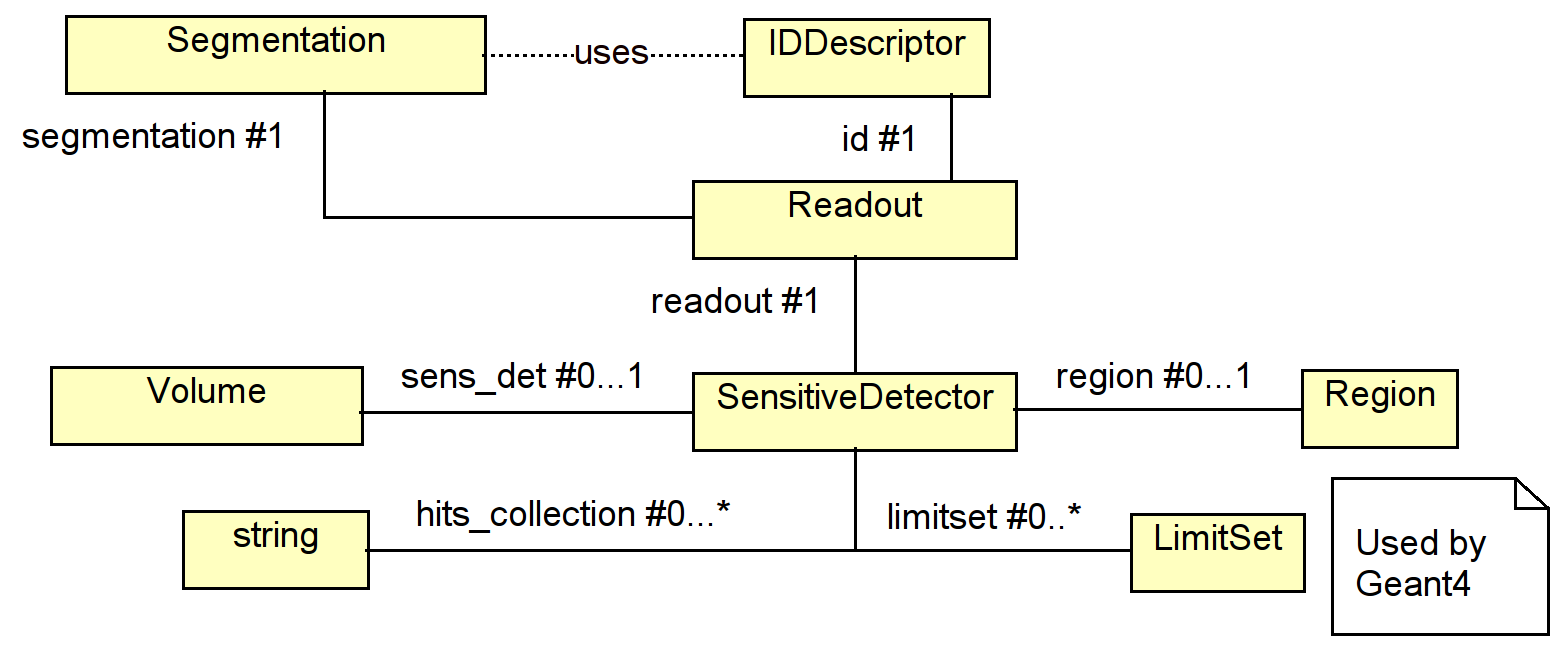
\includegraphics[width=140mm] {DD4hep-sensitive-detectors}
    \caption{The structure of DD4hep sensitive detectors.}
    \label{fig:dd4hep-sensitive-detectors}
  \end{center}
  \vspace{-0.6cm}
\end{figure}

Sensitive detector objects are automatically creating using the information of the \texttt{<readout>} section of the \texttt{XML} file if a subdetector is sensitive and references a valid readout entry. In the detector constructor (or any time later) clients  may add additional information to a sensitive detector object using  an extension mechanism similar to the extension mechanism for  detector elements mentioned earlier.

Volumes may be shared and reused in several placements. In the parallel hierarchy of detector elements as shown in Figure~\ref{fig:dd4hep-hierarchies}, the detector elements may reference unambiguously the volumes of their respective placements, but not the reverse. However, the sensitive detector setup is a single instance per subdetector. Hence it may be referenced by all sensitive Volumes of one subdetector. In the following chapters the access to the readout structure is described.

\section{Description of the Readout Structure}
\label{sec:dd4hep-manual-readout-description}

The \texttt{Readout} class describes the detailed structure of a sensitive volume. The for example may be the layout of strips or pixels in a silicon detector i.e. the description of entities which would not be modeled using individual volumes and placements though this would theoretically  feasible. Each sensitive element is segmented according to the \texttt{Segmentation} object and hits resulting from energy depositions in the sensitive volume are  encoded using the \texttt{IDDescriptor} object.

\begin{figure}[h]
  \begin{center}
    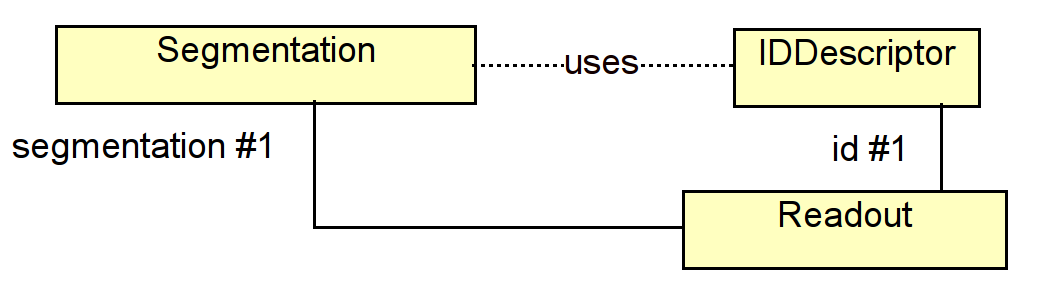
\includegraphics[width=100mm] {DD4hep-readout}
    \caption{The basic components to describe the \texttt{Readout} structure
    of a subdetector. }
    \label{fig:dd4hep-sensitive-detectors}
  \end{center}
  \vspace{-0.6cm}
\end{figure}

\subsection{CellID Descriptors}
\label{sec:dd4hep-manual-readout-iddescriptors}

\texttt{IDDescriptor}s define the encoding of sensitive volumes to uniquely identify the location of the detector response. The encoding defines a bit-field with the length of 64 bits. The first field is mandatory called \texttt{system} and identifies the subdetector. All other fields define the other volumes in the hierarchy. The high bits are not necessarily mapped to small daughter volumes, but may simply identify a logical segmentation such as the \texttt{strip} \texttt{number} within a wafer of a vertex detector as shown in the following \texttt{XML} snippet: 
\begin{minted}[frame=single,framesep=3pt,breaklines=true,tabsize=2,linenos,fontsize=\small]{xml}
<readouts>
  <readout name="SiVertexEndcapHits">
    <id>system:8,barrel:3,layer:4,module:14,sensor:2,side:32:-2,strip:24</id>
  </readout>
<readouts>
\end{minted}
These identifiers are the data input to  \texttt{segmentation classes}~\ref{sec:dd4hep-manual-readout-segmentations}, which define a user friendly API to en/decode the detector response.

\subsection{Segmentations}
\label{sec:dd4hep-manual-readout-segmentations}

Segmentations define the user API to the low level interpretation of the energy deposits in a subdetector. For technical reasons and partial religious reasons are the segmentation implementation not part of the DD4hep  toolkit, but an independent package call \texttt{DDSegmentation}. Though the usage is an integral part of DD4hep.

\subsection{Volume Manager}
The \texttt{VolumeManager} is a tool to seek a look-up table of placements of  sensitive volumes and their corresponding unique volume identifier, the \texttt{cellID}. The volume manager analyzes - once the geometry is closed - the hierarchical tree and stores the various placements in the hierarchy with respect to their identifiers. In other words the the tree is  reused volumes shown e.g. in Figure~\ref{fig:dd4hep-hierarchies} is degenerated  according to the full paths of the various volumes. This  use case is very common to reconstruction and analysis applications whenever a given raw-data (aka ``hit'') element must be related to its geometrical location.

Figure~\ref{fig:dd4hep-user-manual-volmgr} shows the design diagram of this component:
\begin{figure}[h]
  \begin{center}
    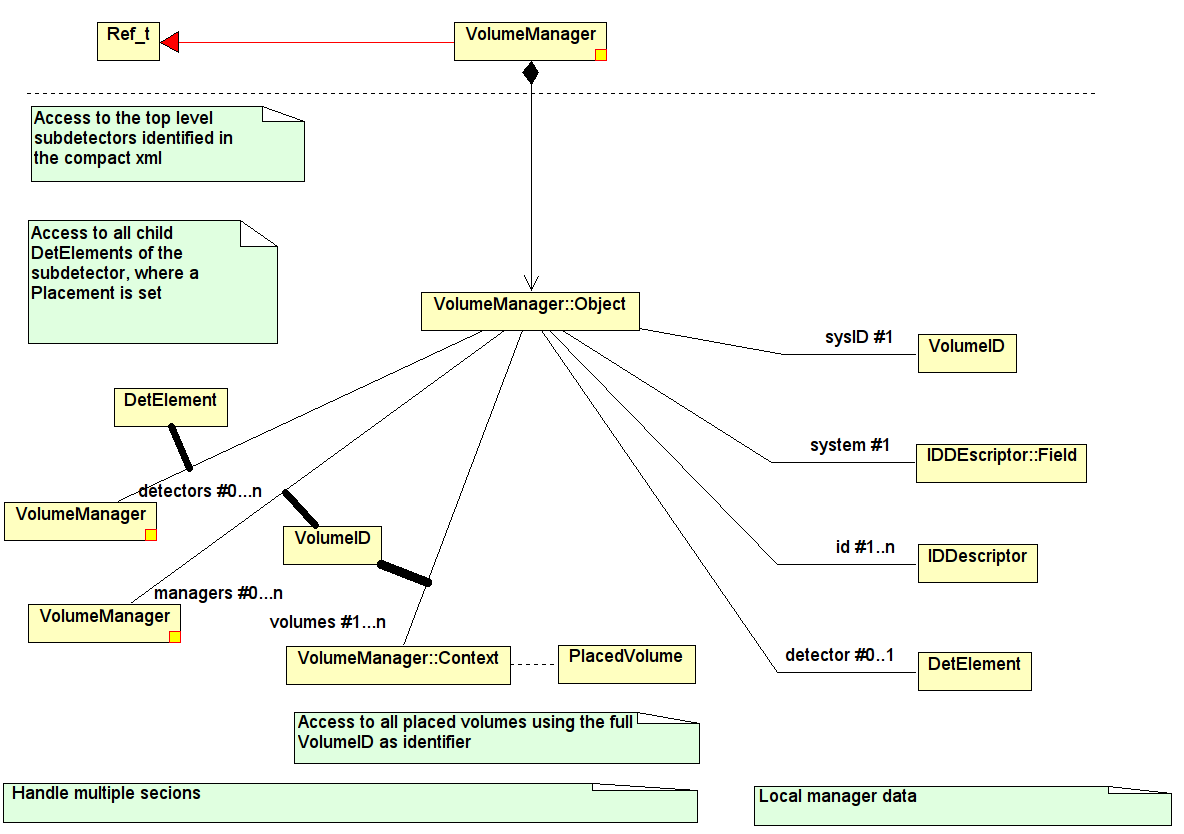
\includegraphics[width=170mm] {DD4hep-volmgr}
    \caption{Extensions may be attached to common Detector Elements which 
             extend the functionality of the common DetElement 
             class and support e.g. caching of precomputed values.}
    \label{fig:dd4hep-user-manual-volmgr}
  \end{center}
\end{figure}

To optimize the access of complex subdetector structures, is the volume-identifier map split and the volumes of each each subdetector is stored in a separate map. This optimization however is transparent to clients. The following code extract from the header files lists the main client routines to extract volume information given a known \texttt{cellID}:
\begin{minted}[frame=single,framesep=3pt,breaklines=true,tabsize=2,linenos,fontsize=\small]{c++}
  /// Lookup the context, which belongs to a registered physical volume.
  Context* lookupContext(VolumeID volume_id) const;
  /// Lookup a physical (placed) volume identified by its 64 bit hit ID
  PlacedVolume lookupPlacement(VolumeID volume_id) const;
  /// Lookup a top level subdetector detector element 
  /// according to a contained 64 bit hit ID
  DetElement lookupDetector(VolumeID volume_id) const;
  /// Lookup the closest subdetector detector element in the hierarchy 
  /// according to a contained 64 bit hit ID
  DetElement lookupDetElement(VolumeID volume_id) const;
  /// Access the transformation of a physical volume to the world coordinate system
  const TGeoMatrix& worldTransformation(VolumeID volume_id) const;
\end{minted}


\subsection{Static Electric and Magnetic Fields}
\label{sec:dd4hep-manual-static-fields}

The generic field is described by a structure of any field type (electric or magnetic) with field components in Cartesian coordinates. The overlay field is the sum of several magnetic of electric field components
and the resulting field vectors are computed by the vector addition of the individual components. The available components are described in the following. If necessary new field implementations may be added at any time: they are  instantiated when necessary by the factory mechanism. Fields are described in the compact model within the {\texttt{<fields>}} tags the following example shows:
\begin{minted}[frame=single,framesep=3pt,breaklines=true,tabsize=2,linenos,fontsize=\small]{xml}
  <fields>
    <field name="MyMagnet" type="solenoid"  .... />
  </fields>
\end{minted}
The actual components are defined one by one within the {\texttt{<field>}} tags.

Constant Electric or Magnetic Fields are defined as follows:
\begin{minted}[frame=single,framesep=3pt,breaklines=true,tabsize=2,linenos,fontsize=\small]{xml}
  <field  name="MyMagnet" type="ConstantField" field="electric">
    <strength x="x-val" y="y-val" z="z-val"/>
  </field>
\end{minted}
The {\texttt{field}} attribute accepts take the values {\texttt{[electric,magnetic]}} depending on its nature.

Magnetic Dipoles are defined as follows:
\begin{minted}[frame=single,framesep=3pt,breaklines=true,tabsize=2,linenos,fontsize=\small]{c++}
  <field name="MyMagnet" type="DipoleMagnet"
         rmax="50*cm"
         zmin="0*cm"
         zmax="50*cm">
         <dipole_coeff>1.0*tesla</dipole_coeff>
         <dipole_coeff>0.1*tesla/pow(cm,1)</dipole_coeff>
         <dipole_coeff>0.01*tesla/pow(cm,2)</dipole_coeff>
  </field>
\end{minted}

Magnetic Multipole Fields are developed according to their  approximation using the multipole coefficients. The dipole is assumed to be horizontal as it is used for bending beams in large colliders
i.e. the dipole field lines are vertical.

The different field components are given by:  
\begin{eqnarray*}
B_{x}^{\mathrm{norm}} &=& \frac{cp}{e} \sum_{m=1}^{\frac{n}{2}} (-1)^{m-1} \; C_n \frac{ x^{n-2 m} \; y^{2 m-1} }{ (n-2 m)!(2 m-1)! } \quad, \\
B_{y}^{\mathrm{norm}} &=& \frac{cp}{e} \sum_{m=0}^{\frac{n-1}{2}} (-1)^m \; C_n \frac{ x^{n-2 m-1} \; y^{2 m} }{ (n-2 m-1)! (2 m)! } \quad, \\
B_{x}^{\mathrm{skew}} &=& \frac{cp}{e} \sum_{m=0}^{\frac{n-1}{2}} (-1)^m \; S_n \frac{ x^{n-2 m-1} \; y^{2 m} }{ (n-2 m-1)! (2 m)! } \quad, \\
B_{y}^{\mathrm{skew}} &=& \frac{cp}{e} \sum_{m=1}^{\frac{n}{2}} (-1)^m \; S_n \frac{ x^{n-2 m} \; y^{2 m-1} }{ (n-2 m)! (2 m-1)! }\quad.
\end{eqnarray*}
With $C_n$ being ``normal multipole coefficients'' and $S_n$ the ``skew multipole coefficients''. The maximal moment used is the octopole moment. The lower four moments are used
to describe the magnetic field:
\begin{itemize}
\item Dipole (n=1):
    \begin{eqnarray*}
        B_x &=& S_1\quad, \\
        B_y &=& C_1\quad, \\
        B_z &=& constant\quad.
    \end{eqnarray*}
\item Quadrupole (n=2):
    \begin{eqnarray*}
        B_x &=& C_2 y+S_2 x\quad, \\
        B_y &=& C_2 x-S_2 y\quad.
    \end{eqnarray*}
\item Sextupole (n=3):
    \begin{eqnarray*}
        B_x         &=& C_3 x y+\frac{S_3 x^2}{2}-\frac{S_3 y^2}{2}\quad, \\
        B_y         &=& \frac{C_3 x^2}{2}-\frac{C_3 y^2}{2}-S_3 x y\quad.
    \end{eqnarray*}

\item Octopole (n=4):
    \begin{eqnarray*}
        B_x &=& \frac{1}{2} C_4 x^2 y-\frac{C_4 y^3}{6}+\frac{S_4 x^3}{6}-\frac{1}{2} S_4 x y^2\quad,\\
        B_y &=& \frac{C_4 x^3}{6}-\frac{1}{2} C_4 x y^2-\frac{1}{2} S_4 x^2 y+\frac{S_4 y^3}{6}\quad.
    \end{eqnarray*}
\end{itemize}
The defined field components only apply within the shape 'volume'. If 'volume' is an invalid shape (i.e. not defined), then the field components are valid throughout the 'universe'.

The magnetic multipoles are defined as follows:
\begin{minted}[frame=single,framesep=3pt,breaklines=true,tabsize=2,linenos,fontsize=\small]{xml}
<field name="MyMagnet" type="MultipoleMagnet">
  <position x="0" y="0" z="0"/>
  <rotation x="pi" y="0" z="0"/>
  <shape type="shape-constructor-type" .... args .... >
  <coefficient coefficient="coeff(n=1)" skew="skew(n=1)"/>
  .... maximum of 4 coefficients ....
  <coefficient coefficient="coeff(n=4)" skew="skew(n=4)"/>
</field>
\end{minted}
The shape defines the geometrical coverage of the multipole  field in the origin (See section~\ref{dd4hep-basic-shapes} for details).  This shape may then be transformed to the required location in the detector area using the position  and the rotation elements, which define this transformation.


\section{Detector Constructors}
\label{sec:dd4hep-manual-detector-constructors}

The creation of appropriate detector constructors is the main work of a client defining his own detector. The detector constructor is a fragment of code in the  form of a routine, which return a handle to the created subdetector \texttt{DetElement} object.

Knowing that detector constructors are the main work items of clients significant  effort was put in place to ease and simplify this procedure as much as possible in order to obtain readable, still compact code hopefully easy to maintain. The interfaces to all objects, \texttt{XML} accessors, shapes, volumes etc. which were  discussed above were optimized to support this intention.

To illustrate the anatomy of such a constructor the following code originating from an existing SiD detector concept will be analyzed. The example starts with the \texttt{XML} input data. Further down this section the code is shown with a detailed description of every relevant line. The object to be build is a subdetector representing a layered calorimeter,  where each layer consists of a number of slices as shown in the \texttt{XML} snippet. These layers are then repeated a number of times.

The \texttt{XML} snippet describing the subdetector properties:
\begin{minted}[frame=single,framesep=3pt,breaklines=true,tabsize=2,linenos,fontsize=\small]{xml}
  <detector id="13" name="LumiCal" reflect="true" type="CylindricalEndcapCalorimeter" 
            readout="LumiCalHits" vis="LumiCalVis" calorimeterType="LUMI">
    <comment>Luminosity Calorimeter</comment>
    <dimensions inner_r = "LumiCal_rmin" inner_z = "LumiCal_zmin" outer_r = "LumiCal_rmax" />
    <layer repeat="20" >
      <slice material = "TungstenDens24" thickness = "0.271*cm" />
      <slice material = "Silicon" thickness = "0.032*cm" sensitive = "yes" />
      <slice material = "Copper"  thickness = "0.005*cm" />
      <slice material = "Kapton"  thickness = "0.030*cm" />
      <slice material = "Air"     thickness = "0.033*cm" />
    </layer>
    <layer repeat="15" >
      <slice material = "TungstenDens24" thickness = "0.543*cm" />
      <slice material = "Silicon" thickness = "0.032*cm" sensitive = "yes" />
      <slice material = "Copper"  thickness = "0.005*cm" />
      <slice material = "Kapton"  thickness = "0.030*cm" />
      <slice material = "Air"     thickness = "0.033*cm" />
    </layer>
  </detector>
\end{minted}

The \texttt{C++} code snippet interpreting the \texttt{XML} data and expanding the geometry:
\begin{minted}[frame=single,framesep=3pt,breaklines=true,tabsize=2,linenos,fontsize=\small]{c++}
#include "DD4hep/DetFactoryHelper.h"
#include "XML/Layering.h"

using namespace std;
using namespace dd4hep;

static Ref_t create_detector(Detector& lcdd, xml_h e, SensitiveDetector sens)  {
  xml_det_t  x_det     = e;
  string     det_name  = x_det.nameStr();
  bool       reflect   = x_det.reflect();
  xml_dim_t  dim       = x_det.dimensions();
  double     zmin      = dim.inner_z();
  double     rmin      = dim.inner_r();
  double     rmax      = dim.outer_r();
  double     totWidth  = Layering(x_det).totalThickness();
  double     z         = zmin;
  Material   air       = lcdd.air();
  Tube       envelope   (rmin,rmax,totWidth,0,2*M_PI);
  Volume     envelopeVol(det_name+"_envelope",envelope,air);
  int        layer_num = 1;
  PlacedVolume pv;

  // Set attributes of slice
  for(xml_coll_t c(x_det,_U(layer)); c; ++c)  {
    xml_comp_t x_layer = c;
    double layerWidth = 0;
    for(xml_coll_t l(x_layer,_U(slice)); l; ++l)
      layerWidth += xml_comp_t(l).thickness();

    for(int i=0, m=0, repeat=x_layer.repeat(); i<repeat; ++i, m=0)  {
      double     zlayer = z;
      string     layer_name = det_name + _toString(layer_num,"_layer%d");
      Volume     layer_vol(layer_name,Tube(rmin,rmax,layerWidth),air);
        
      for(xml_coll_t l(x_layer,_U(slice)); l; ++l, ++m)  {
        xml_comp_t x_slice = l;
        double     w = x_slice.thickness();
        string     slice_name = layer_name + _toString(m+1,"slice%d");
        Material   slice_mat  = lcdd.material(x_slice.materialStr());
        Volume     slice_vol (slice_name,Tube(rmin,rmax,w),slice_mat);
          
        if ( x_slice.isSensitive() )  {
          sens.setType("calorimeter");
          slice_vol.setSensitiveDetector(sens);
        }
        slice_vol.setAttributes(lcdd, x_slice.regionStr(), x_slice.limitsStr(), x_slice.visStr());
        pv = layer_vol.placeVolume(slice_vol, Position(0,0,z-zlayer-layerWidth/2+w/2));
        pv.addPhysVolID("slice",m+1);
        z += w;
      }
      layer_vol.setVisAttributes(lcdd,x_layer.visStr());
      Position layer_pos(0,0,zlayer-zmin-totWidth/2+layerWidth/2);
      pv = envelopeVol.placeVolume(layer_vol,layer_pos);
      pv.addPhysVolID("layer",layer_num);
      ++layer_num;
    }
  }
  // Set attributes of slice
  envelopeVol.setAttributes(lcdd, x_det.regionStr(), x_det.limitsStr(), x_det.visStr());

  DetElement   sdet(det_name,x_det.id());
  Volume       motherVol = lcdd.pickMotherVolume(sdet);
  PlacedVolume phv = motherVol.placeVolume(envelopeVol,Position(0,0,zmin+totWidth/2));
  phv.addPhysVolID("system",sdet.id()).addPhysVolID("barrel",1);
  sdet.setPlacement(phv);
  if ( reflect )   {
    phv=motherVol.placeVolume(envelopeVol, Transform3D(RotationZ(M_PI), Position(0,0,-zmin-totWidth/2)));
    phv.addPhysVolID("system",sdet.id()).addPhysVolID("barrel",2);
  }
  return sdet;
}

DECLARE_DETELEMENT(CylindricalEndcapCalorimeter,create_detector);
\end{minted}
{\small
\begin{tabular} {p{0.1\linewidth}|p{0.9\linewidth}}
\hline \\
1 & The include file DetFactoryHelper.h includes all utilities to extract \texttt{XML} information together with the appropriate type definition.\\
4-5 & Convenience shortcut to save us a lot of typing.\\
7 & The entry point to the detector constructor. This routine shall be called by the plugin mechanism.\\
8 & The functionality of the raw \texttt{XML} handle \texttt{xml\_h} is rather limited. A simple assignment to a \texttt{XML} detector object gives us all the functionality we need.\\
9--10 & Extracting the sub-detector name and properties from the xml handle.\\
11--16 & Access the \texttt{dimension} child-element from the \texttt{XML} subtree, access the element's attributes and precompute values used later.\\
17 & Retrieve a reference to the ``air'' material from \texttt{Detector}.\\
18--19 & Construct the envelope volume shaped as a tube made out of air.\\
24 & Now the detector can be built: We loop over all layers types and over each layer type as often as necessary (attribute: repeat).The \texttt{XML} collection object will return all child elements of \texttt{x\_det}with a tag-name ``layer''.  Note the macro \texttt{\_U(layer)}: When using Xerces-C as an \texttt{XML} parser, it will expand to the reference to an object containing the unicode value of the string ``layer''. The full list of predefined tag names can be found in the include file \texttt{XML/UnicodeValues.h}.If a user tag is not part in the precompiled tag list, the corresponding Unicodestring may be created with the macro \texttt{\_Unicode(layer)} or \texttt{Unicode("layer")}.\\
25 & Convenience assignment to extract attributes of the layer element.\\
26--28 & Compute total layer width.\\
30 & Create \texttt{repeat} number of layers of the same type.\\
31-33 & Create the named envelope volume with a tube shape containing all slices of this layer.\\
35-50 & Create the different layer-slices with a tube shape and the corresponding material as indicated in the \texttt{XML} data.\\
42-45 & If the slice is sensitive i.e. is instrumented and supposed to deliver signals from particle passing, the sensitive detector component of this detector needs to be attached to the slice.\\
46 & Set visualization and Geant4 attributes to the slice volume. If the attributes are not present, they will be ignored.\\
47 & Now the created slice volume will be placed inside the mother, the layer envelope at the correct position. This operation results in the creation of a \texttt{PlacedVolume}.\\
48 & It identify uniquely every slice within the layer an identifier (here the number of the created slice) is attached. This identifier must be present in the bitmap defined by the \texttt{IDDescriptor} of this subdetector.\\
52-55 & Same as 46-48, but now the created layer volume is placed in the envelope of the entire subdetector.\\
59 & Set envelope attributes.\\
61 & Construct the main detector element of this subdetector.This will be the unique entry point to access any information of the subdetector. {\textbf{Note:}} the subdetector my consist of a hierarchy of detector elements.For example each layer could be described by its own \texttt{DetElement} and all layer-\texttt{DetElement} instances being children of the subdetector instance.\\
62-62 & Place the subdetector envelope into its mother (typically the top level (world) volume).\\
64-65 & Add the missing \texttt{IDDescriptor} identifiers to complete the bitmap.\\
66 & Store the placement in the subdetector detector element in order to make it available to later clients of this \texttt{DetElement}. \\
67-69 & Endcap calorimeters typically are symmetric i.e. an endcap is located on each side of the barrel. To easy such reflections the entire endcap structure can be copied and placed again. \\
70 & All done. Return the created subdetector element to the caller for registration. \\ 
73 & \textbf{Very important:} Without the registration of the construction function to the framework, the corresponding plugin will not be found. The macro has two arguments: firstly the plugin name which is identical to the detector type in the \texttt{XML} snippet and secondly the function to be called at construction time.
\end{tabular}
}
\section{Tools and Utilities}


\subsection{Geometry Visualization}
\label{sec:dd4hep-manual-geometry-visualization}

Visualizing the geometry is an important tool to debug and validate the constructed detector. Since DD4hep uses the \texttt{ROOT} geometry package, all visualization tools from ROOT are automatically supported. This is in the first place the OpenGL canvas of \texttt{ROOT} and all elaborated derivatives thereof such as  event displays etc. Figure~\ref{fig:dd4hep-user-manual-visualization-subdetector} shows as an example the subdetector example from the \texttt{SiD} detector design discussed in section~\ref{sec:dd4hep-manual-detector-constructors}.
\begin{figure}[h]
  \begin{center}
    \begin{tabular}{l r}
      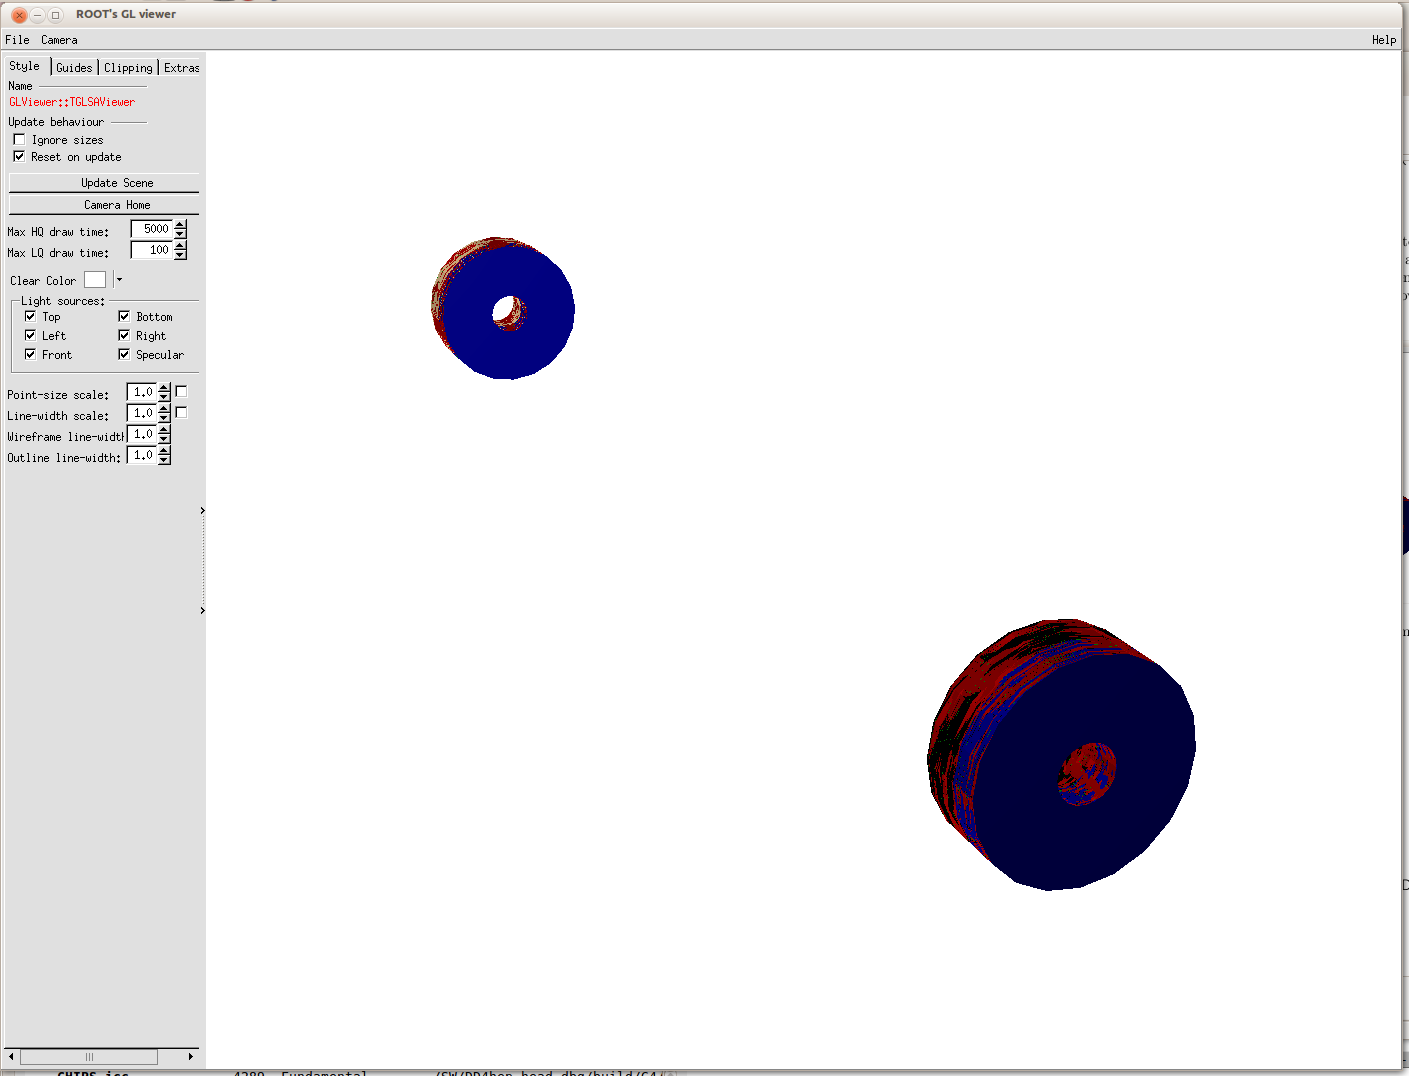
\includegraphics[width=80mm] {DD4hep-Lumical} &
      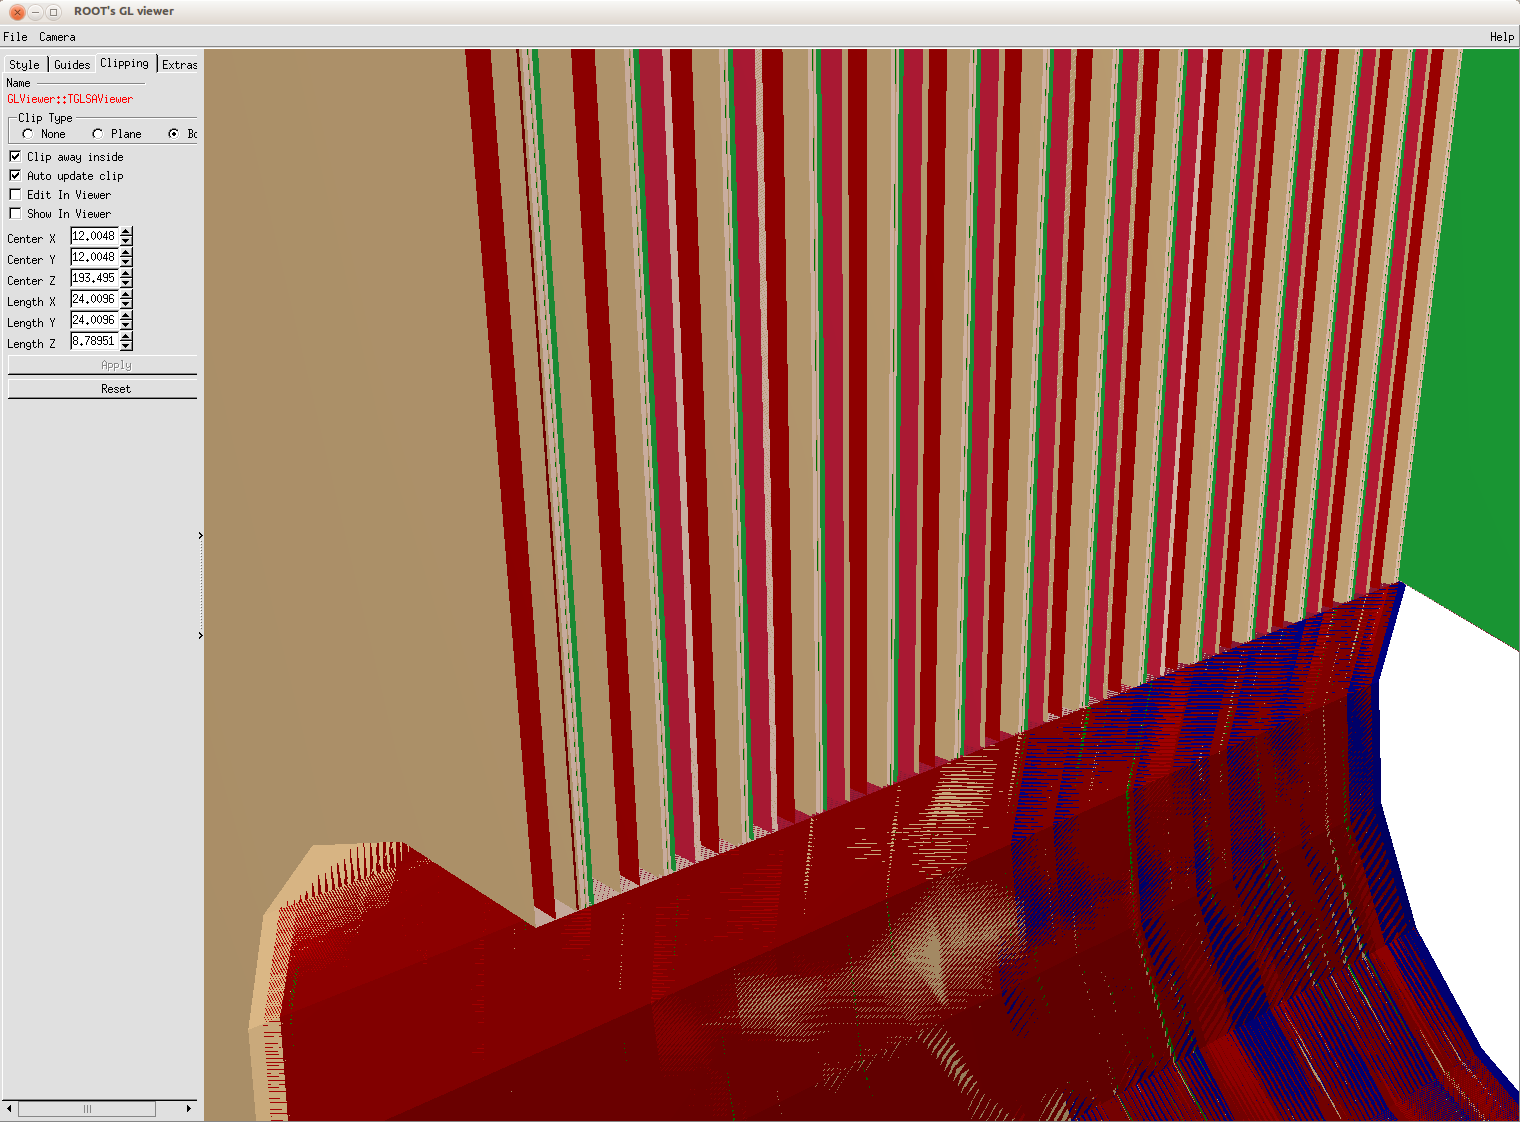
\includegraphics[width=80mm] {DD4hep-Lumical-detailed} \\
    \end{tabular}
    \caption{Geometry visualization using the ROOT OpenGL plugin.
        To the left the entire luminosity calorimeter is shown,
        at the right the detailed zoomed view with clipping to 
        access the internal layer and slice structure.}
    \label{fig:dd4hep-user-manual-visualization-subdetector}
  \end{center}
\end{figure}

The command to create the display is part of the DD4hep release:
\begin{minted}[frame=single,framesep=3pt,breaklines=true,tabsize=2,linenos,fontsize=\small]{bash}
$> geoDisplay -compact <path to the \texttt{XML} file containing the detector description>

 DD4hepGeometryDisplay -opt [-opt]                                                  
        -compact       <file>       Specify the compact geometry file              
                     [REQUIRED]     At least one compact geo file is required!     
        -build_type <number/string> Specify the build type                         
                     [OPTIONAL]     MUST come immediately after the -compact input.
                                    Default for each file is: BUILD_DEFAULT [=1]   
                                    Allowed values: BUILD_SIMU [=1], BUILD_RECO [=2] or BUILD_DISPLAY [=3]
        -destroy     [OPTIONAL]     Force destruction of the Detector instance         
                                    before exiting the application                 
        -volmgr      [OPTIONAL]     Load and populate phys.volume manager to       
                                    check the volume ids for duplicates etc.       
        -print      <number/string> Specify output level. Default: INFO(=3)        
                     [OPTIONAL]     Allowed values: VERBOSE(=1), DEBUG(=2),        
                                    INFO(=3), WARNING(=4), ERROR(=5), FATAL(=6)    
                                    The lower the level, the more printout...      
        -load_only   [OPTIONAL]     Dry-run to only load geometry without     
                                    starting the display.                      
\end{minted}


\subsection{Geometry Conversion}
\label{sec:dd4hep-manual-geometry-conversion}

\texttt{ROOT} \texttt{TGeo} is only one representation of a detector geometry. Other applications may require other representation. In particular two other are worth mentioning:
\begin{itemize}
\item \texttt{Detector}~\cite{Gaede:81331} the geometry representation used to simulate the ILC detector design with the \texttt{slic} application.
\item \texttt{GDML}~\cite{Chytracek:2006be} a geometry markup language understood by Geant4 and \texttt{ROOT}.
\end{itemize}
Both conversions are supported in DD4hep with the geoConverter application:
\begin{minted}[frame=single,framesep=3pt,breaklines=true,tabsize=2,linenos,fontsize=\small]{bash}
  geoConverter -opt [-opt]                                                
        Action flags:               Usage is exclusive, 1 required!           
        -compact2lcdd               Convert compact xml geometry to lcdd.     
        -compact2gdml               Convert compact xml geometry to gdml.     
        -compact2vis                Convert compact xml to visualisation attrs

        -input  <file>  [REQUIRED]  Specify input file.                       
        -output <file>  [OPTIONAL]  Specify output file.                      
                                    if no output file is specified, the output
                                    device is stdout.                         
        -ascii          [OPTIONAL]  Dump visualisation attrs in csv format.   
                                    [Only valid for -compact2vis]             
\end{minted}

\subsection{Overlap checking}
\label{sec:dd4hep-manual-overlap-checking}

Overlap checks are an important tool to verify the consistency of the  implemented geometrical design. As in the real world, where overlaps are  impossible, also simulated geometries may not have overlaps. In simulation overlaps tend to create particle reflections possibly leading to infinite loops.
\begin{minted}[frame=single,framesep=3pt,breaklines=true,tabsize=2,linenos,fontsize=\small]{bash}
    python <install>/DD4hep/bin/checkOverlaps.py --help
    Usage: checkOverlaps.py [options]

    Check TGeo geometries for overlaps.

    Options:
      -h, --help                        show this help message and exit
      -c <FILE>, --compact=<FILE>       Define LCCDD style compact xml input
      -p <boolean>, --print=<boolean>   Print overlap information to standard output
                                        (default:True)
      -q, --quiet                       Do not print (disable --print)
      -t <double number>, --tolerance=<double number>
                                        Overlap checking tolerance. Unit is in [mm].
                                        (default:0.1 mm)
      -o <string>, --option=<string>    Overlap checking option ('' or 's')
\end{minted}

\subsection{Geometry checking}
\label{sec:dd4hep-manual-geometry-checking}

Perform extensive geometry checks. For details and up to date information  please refer to the ROOT documentation of the class {\texttt{TGeoManager}}:
\begin{itemize}
\item Member function \texttt{TGeoManager::CheckGeometry} and 
\item Member function \texttt{TGeoManager::CheckGeometryFull}
\end{itemize}

\begin{minted}[frame=single,framesep=3pt,breaklines=true,tabsize=2,linenos,fontsize=\small]{bash}
    python <install>DD4hep/bin/checkGeometry.py --help
    Usage: checkGeometry.py [options]

    TGeo Geometry checking.

    Options:
      -h, --help                            show this help message and exit
      -c <FILE>, --compact=<FILE>           Define LCCDD style compact xml input
      -f <boolean>, --full=<boolean>        Full geometry checking
      -n <integer>, --ntracks=<integer>     Number of tracks [requires 'full']
      -x <double>, --vx=<double>            X-position of track origine vertex [requires 'full']
      -y <double>, --vy=<double>            Y-position of track origine vertex [requires 'full']
      -z <double>, --vz=<double>            Z-position of track origine vertex [requires 'full']
      -o <string>, --option=<string>        Geometry checking option default:ob
\end{minted}

The full geometry check performs the \texttt{TGeoManager:CheckGeometryFull} following actions:
\begin{itemize}
\item if option contains 'o': Optional overlap checkings (by sampling and by mesh).
\item if option contains 'b': Optional boundary crossing check + timing per volume.
\end{itemize}
\begin{description}
\item[STAGE 1] extensive overlap checking by sampling per volume. Stdout need to be checked by user to get report, then \texttt{TGeoVolume::CheckOverlaps(0.01, "s")} can be called for the suspicious volumes.
\item[STAGE 2] normal overlap checking using the shapes mesh - fills the list of overlaps.
\item[STAGE 3:] shooting NTRACKS rays from vertex \texttt{(vx,vy,vz)} and counting the total number of crossings per volume (rays propagated from boundary to boundary until geometry exit). Timing computed and results stored in a histogram.
\item[STAGE 4:] shooting 1 mil. random rays inside EACH volume and calling FindNextBoundary() + Safety() for each call. The timing is normalized by the number of crossings computed at stage 2 and presented as percentage. One can get a picture on which are the most ``burned'' volumes during transportation from geometry point of view. Another plot of the timing per volume vs. number of daughters is produced.
\end{description}

\subsection{Directional Material Scans}
\label{sec:dd4hep-manual-directional-material-scans}

Print the materials on a straight line between the two given points:
\begin{minted}[frame=single,framesep=3pt,breaklines=true,tabsize=2,linenos,fontsize=\small]{bash}
materialScan
 usage: print_materials compact.xml x0 y0 z0 x1 y1 z1 
        -> prints the materials on a straight line between the two given points ( unit is cm) 
\end{minted}
\texttt{materialScan} uses the python bindings provided by Geant4 and may be not  always availible. Alternatively the command \texttt{print\_materials} may be used, which does not use the python binding, but produces less pretty output.


\subsection{Plugin Test Program}
\label{sec:dd4hep-manual-plugin-test}

The plugin tester loads a given geometry and the executes a plugin defined at the command line. The main purpose of this program is to quickly  invoke new detector plugins while developing. The arguments for this  program are:
\begin{minted}[frame=single,framesep=3pt,breaklines=true,tabsize=2,linenos,fontsize=\small]{bash}
    geoPluginRun -opt [-opt]                                                
    
        -plugin <name>  [REQUIRED]  Plugin to be executed and applied.        
        -input  <file>  [OPTIONAL]  Specify geometry input file.              
        -build_type <number/string> Specify the build type                         
                     [OPTIONAL]     MUST come immediately after the -compact input.
                                    Default for each file is: BUILD_DEFAULT [=1]   
                                    Allowed values: BUILD_SIMU [=1], BUILD_RECO [=2] or BUILD_DISPLAY [=3]
        -destroy     [OPTIONAL]     Force destruction of the LCDD instance         
                                    before exiting the application                 
        -volmgr      [OPTIONAL]     Load and populate phys.volume manager to       
                                    check the volume ids for duplicates etc.       
        -print      <number/string> Specify output level. Default: INFO(=3)        
                     [OPTIONAL]     Allowed values: VERBOSE(=1), DEBUG(=2),        
                                    INFO(=3), WARNING(=4), ERROR(=5), FATAL(=6)    
                                    The lower the level, the more printout...
\end{minted}
To invoke plugins using this utility is very simple and any number of plugins may be chained
to produce the required result. This is very convenient e.g. to run tests:
\begin{minted}[frame=single,framesep=3pt,breaklines=true,tabsize=2,linenos,fontsize=\small]{bash}
  $> geoPluginRun -input <compact geometry file> \
                  -plugin <plugin-name-1> <plugin-arg-1>  <plugin-arg-2> ....
                  -plugin <plugin-name-2> <plugin-arg-1>  <plugin-arg-2> ....
                  -plugin <plugin-name-3> <plugin-arg-1>  <plugin-arg-2> ....
                  ....
\end{minted}

\section{Standard Plugins}
\label{sec:dd4hep-manual-standard-plugins}
These plugins are partially used by DD4hep itself and are invoked from therein,
but can as well be initiated from the above mentioned plugin test program.

\subsection{Geometry Display}
\label{sec:dd4hep-manual-plugin-geometry-display}

This plugin may be used to invoke the geometry display and start the ROOT interpreter:
\begin{minted}[frame=single,framesep=3pt,breaklines=true,tabsize=2,linenos,fontsize=\small]{bash}
    Usage: -plugin DD4hep_GeometryDisplay  -arg [-arg]                                
  	       Invoke the ROOT geometry display using the factory mechanism.                
             -detector <string> Top level DetElement path. Default: '/world'                
             -option   <string> ROOT Draw option.    Default: 'ogl'                         
             -level    <number> Visualization level  [TGeoManager::SetVisLevel]  Default: 4 
             -visopt   <number> Visualization option [TGeoManager::SetVisOption] Default: 1       
             -load              Only load the geometry. Do not invoke the display          
             -help              Print this help output         

    For details see also: DDCore/src/plugins/StandardPlugins.cpp
\end{minted}

\subsection{Execute a Function in a Library}
\label{sec:dd4hep-manual-plugin-execute-function}

Plugin to invoke a C function in a library. The plugin automatically loads the library and
executes the function. The function may not require arguments. The function is identified by it's 
linker name. Hence, to not need to deal with linker name mangling export such functions
with \texttt{extern ``C''}.
\begin{minted}[frame=single,framesep=3pt,breaklines=true,tabsize=2,linenos,fontsize=\small]{bash}
    Usage: -plugin DD4hep_Function -arg [-arg]                                 
             Execute a function without arguments inside a library.     
           -library   <string>    Library to be loaded                    
           -function  <string>    name of the entry point to be executed. 

    For details see also: DDCore/src/plugins/StandardPlugins.cpp
\end{minted}

\subsection{Start the ROOT Interpreter}
\label{sec:dd4hep-manual-plugin-root-interpreter}

To trigger the start of the ROOT interpreter, invoke the plugin. Additional argumens are 
assumed to be command, which should be evaluated.
\begin{minted}[frame=single,framesep=3pt,breaklines=true,tabsize=2,linenos,fontsize=\small]{bash}
    Usage: -plugin DD4hep_Rint -arg [-arg]                                 
             Start the ROOT interpreter. Optionally process one or several commands.

    For details see also: DDCore/src/plugins/StandardPlugins.cpp
\end{minted}

\subsection{Start the DD4hep UI}
\label{sec:dd4hep-manual-plugin-dd4hep-ui}

The DD4hep UI is a mediator to interactively interact more easily with the DD4hep instance from the 
ROOT command prompt. See the defintition file \texttt{DDCore/include/DD4hep/DD4hepUI.h} for details.
An instance of the \texttt{DD4hepUI} class is generated and made availible to ROOT by the global pointer
gDD4hepUI. Any argument is ignored.
\begin{minted}[frame=single,framesep=3pt,breaklines=true,tabsize=2,linenos,fontsize=\small]{bash}
    Usage: -plugin DD4hep_InteractiveUI

    For details see also: DDCore/src/plugins/StandardPlugins.cpp
\end{minted}

\subsection{Dump GDML Tables of the TGeoManager}
\label{sec:dd4hep-manual-plugin-dump-gdml-tables}

The plugin simply dumps the GDML tables associated to the \texttt{TGeoManager} instance to stdout.
Useful to verify the parsed conent.
Any argument is ignored.
\begin{minted}[frame=single,framesep=3pt,breaklines=true,tabsize=2,linenos,fontsize=\small]{bash}
    Usage: -plugin DD4hep_Dump_GDMLTables

    For details see also: DDCore/src/plugins/StandardPlugins.cpp
\end{minted}

\subsection{Dump Optical Surfaces of the TGeoManager}
\label{sec:dd4hep-manual-plugin-dump-optical-surfaces}

The plugin simply dumps the optical surfaces associated to the \texttt{TGeoManager} instance to stdout.
Useful to verify the parsed conent.
Any argument is ignored.
\begin{minted}[frame=single,framesep=3pt,breaklines=true,tabsize=2,linenos,fontsize=\small]{bash}
    Usage: -plugin DD4hep_Dump_OpticalSurfaces

    For details see also: DDCore/src/plugins/StandardPlugins.cpp
\end{minted}

\subsection{Dump Skin Surfaces of the TGeoManager}
\label{sec:dd4hep-manual-plugin-dump-skin-surfaces}

The plugin simply dumps the skin surfaces associated to the \texttt{TGeoManager} instance to stdout.
Useful to verify the parsed conent.
Any argument is ignored.
\begin{minted}[frame=single,framesep=3pt,breaklines=true,tabsize=2,linenos,fontsize=\small]{bash}
    Usage: -plugin DD4hep_Dump_SkinSurfaces

    For details see also: DDCore/src/plugins/StandardPlugins.cpp
\end{minted}

\subsection{Dump Border Surfaces of the TGeoManager}
\label{sec:dd4hep-manual-plugin-dump-border-surfaces}

The plugin simply dumps the border surfaces associated to the TGeoManager instance to stdout.
Useful to verify the parsed conent.
Any argument is ignored.
\begin{minted}[frame=single,framesep=3pt,breaklines=true,tabsize=2,linenos,fontsize=\small]{bash}
    Usage: -plugin DD4hep_Dump_BorderSurfaces

    For details see also: DDCore/src/plugins/StandardPlugins.cpp
\end{minted}

\subsection{Dump the Element/Material Table of the TGeoManager}
\label{sec:dd4hep-manual-plugin-dump-material-table}

The plugin dumps all elements stored in the TGeoManager instance to stdout or to file.
Optionally the output can be generated in XML understood by DD4hep in order to e.g.
export the elements used in the apparatus.
Useful to verify the parsed conent.
\begin{minted}[frame=single,framesep=3pt,breaklines=true,tabsize=2,linenos,fontsize=\small]{bash}
    Usage:  -plugin DD4hep_ElementTable -opt [-opt]
                  -type   <string>    Output format: text or xml
                  -output <file-name> Output file specifier (xml only)

    For details see also: DDCore/src/plugins/StandardPlugins.cpp
\end{minted}
To dump the material table, use the plugin \texttt{DD4hep\_MaterialTable}.

\subsection{Load and Interprete XML file}
\label{sec:dd4hep-manual-plugin-load-xml}

Load and interprete an \texttt{XML} file with DD4hep.
The root tag name of the file defines the factory name to be called
to analyse the content. The optional build type is a flag passed to the
Detector entity and may be used for more detailed interpretation.
\begin{minted}[frame=single,framesep=3pt,breaklines=true,tabsize=2,linenos,fontsize=\small]{bash}
    Usage:  -plugin DD4hep_XMLLoader <file-uri> <build-type>

    For details see also: DDCore/src/plugins/StandardPlugins.cpp
\end{minted}

\subsection{Load and Interprete XML Element}
\label{sec:dd4hep-manual-plugin-process-xml-element}

Interprete a single XML element.
The root tag name of the file defines the factory name to be called
to analyse the content. The optional build type is a flag passed to the
Detector entity and may be used for more detailed interpretation.
This plugin can only be used, since the argument to a pointer to an \texttt{XML::Handle}
is passed.
\begin{minted}[frame=single,framesep=3pt,breaklines=true,tabsize=2,linenos,fontsize=\small]{bash}
    Usage:  -plugin DD4hep_XMLProcessor <pointer-to-xml-element> <build-type>

    For details see also: DDCore/src/plugins/StandardPlugins.cpp
\end{minted}

\subsection{Load and Initialize the DD4hep Volume Manager}
\label{sec:dd4hep-manual-plugin-volume-manager}

To load and initialize the DD4hep volume manager object, use:
\begin{minted}[frame=single,framesep=3pt,breaklines=true,tabsize=2,linenos,fontsize=\small]{bash}
    Usage:  -plugin DD4hep_VolumeManager

    For details see also: DDCore/src/plugins/StandardPlugins.cpp
\end{minted}
Any argument is ignored. Please note: the detector description must be full initialized 
before this plugin may be called. Anything else results in incomplete content.


\subsection{Dump Detector Description to ROOT file}
\label{sec:dd4hep-manual-plugin-save-dd4hep-root}

This plugin saves the full detector description object to a ROOT file 
including geometry and structural setup. Please note, that for reading 
DD4hep is required to resolve the necessary dictionaries. However, this 
method may serve to produce well defined snapshots e.g. for mass production.
\begin{minted}[frame=single,framesep=3pt,breaklines=true,tabsize=2,linenos,fontsize=\small]{bash}
     Usage: -plugin DD4hep_Geometry2ROOT -arg [-arg]
             -output <string>         Output file name.

    For details see also: DDCore/src/plugins/StandardPlugins.cpp
\end{minted}

\subsection{Load Detector Description from ROOT file}
\label{sec:dd4hep-manual-plugin-load-dd4hep-root}

Once saved, load the DD4hep detector description into memory.
\begin{minted}[frame=single,framesep=3pt,breaklines=true,tabsize=2,linenos,fontsize=\small]{bash}
     Usage: -plugin DD4hep_RootLoader -arg [-arg]
             -input <string>         Input file name.

    For details see also: DDCore/src/plugins/StandardPlugins.cpp
\end{minted}

\subsection{Dump Geometry to ROOT file}
\label{sec:dd4hep-manual-plugin-save-geometry-root}

The plugin saves the geometry part of the detector description to ROOT.
Only ROOT is required to read this information.
\begin{minted}[frame=single,framesep=3pt,breaklines=true,tabsize=2,linenos,fontsize=\small]{bash}
    Usage: -plugin DD4hep_Geometry2TGeo -arg [-arg]
             -output <string>         Output file name.

    For details see also: DDCore/src/plugins/StandardPlugins.cpp
\end{minted}

\subsection{Dump DetElement/Volume Tree}
\label{sec:dd4hep-manual-plugin-dump-detelement-volume-tree}

Dump for verification and debugging the \texttt{DetElement} or \texttt{Volume} tree
of the detector description. Both plugin are very similar, once with emphsis on the
ejected \texttt{DetElement} information, once with emphasis on the geometry information.
\begin{minted}[frame=single,framesep=3pt,breaklines=true,tabsize=2,linenos,fontsize=\small]{bash}
   Usage -plugin DD4hep_DetectorDump / DD4hep_DetectorVolumeDump -arg [-arg]

	       --sensitive             Process only sensitive volumes.                                
	        -sensitive             dto.                                                           
	       --no-sensitive          Invert sensitive only flag.                                    
	        -no-sensitive          dto.                                                           
	       --shapes                Print shape information.                                       
	        -shapes                dto.                                                           
	       --positions             Print position information.                                    
	        -positions             dto.                                                           
	       --materials             Print material information.                                    
	        -materials             dto.                                                           
	       --detector    <path>    Process elements only if <path> is part of the DetElement path.
	        -detector    <path>    dto.                                                           
	        -level       <number>  Maximal depth to be explored by the scan                       
	       --level       <number>  dto.                                                           
	        -volids                Print volume identifiers of placements.                        
	       --volids                dto.                                                           

    For details see also: DDCore/src/plugins/StandardPlugins.cpp
\end{minted}

\subsection{Fill DetElement Cache}
\label{sec:dd4hep-manual-plugin-chache-detelement-info}

The DetElement instances may cache on demand the transfomattions of their ideal placements
to the world coordinate system. To fill this cache immediately rather than on demand use this
plugin. Depending on the top element passed, this caching mechanism can also be applied to
some sub-detectors.
\begin{minted}[frame=single,framesep=3pt,breaklines=true,tabsize=2,linenos,fontsize=\small]{bash}
    Usage: -plugin DD4hep_DetElementCache  -arg [-arg]                 
             -detector <string>  Top level DetElement path. Default: '/world'
	     --detector <string> dto.                                        

    For details see also: DDCore/src/plugins/StandardPlugins.cpp
\end{minted}



\section{Shape and Volume Plugins}
\label{sec:dd4hep-manual-shape-plugins}

Shape plugins can be used to create shapes and volumes using uniquely xml constructs without the
need of extra code. Often useful when describing passive objects of an apparatus.
DD4hep supports all commonly used and supported shapes by TGeo, and allows the abstract creation 
of these shapes using the plugin mechanism. We list here the shapes, which are supported by 
the plugin mechanism. The creation of shapes can be triggered using any XML element matching 
a given pattern. The constructor is accessible as follows:

\begin{minted}[frame=single,framesep=3pt,breaklines=true,tabsize=2,linenos,fontsize=\small]{bash}
#include <XML/Utilities.h>

  Detector& det = ...;
  xml::Element element = ...;
  std::string shape_type = "Box";
  Solid solid = dd4hep::xml::createShape(description, shape_type, element);
\end{minted}
where the XML Element \texttt{element} must supply all required information to actually create the 
shape of a given type.
To create shapes with the fectory mechanism, the shape constructors as present in 
\texttt{DDCore/inlude/DD4hep/Shapes.h} must be met.

\subsection{Assembly Shape Construction}
\label{sec:dd4hep-manual-plugin-assembly-shape}

The xml entity 'element' must look like the following: 
\begin{minted}[frame=single,framesep=3pt,breaklines=true,tabsize=2,linenos,fontsize=\small]{bash}
   <some-tag name="my-assembly"  ......further xml-attributes not looked at .... >
        ... further optional xml-elements not looked at .... 
   </some-tag>
\end{minted}
The name attribute is optional. If present the created \texttt{TGeoShapeAssembly} will be given the 
supplied identifier.

\subsection{Scaled Shape Construction}
\label{sec:dd4hep-manual-plugin-scaled-shape}

The xml entity 'element' must look like the following: 
\begin{minted}[frame=single,framesep=3pt,breaklines=true,tabsize=2,linenos,fontsize=\small]{bash}
   <some-tag name="my-solid" x="1.0" y="2.0" z="3.0" ... further xml-attributes not looked at .... >
        <shape>  ......  </shape>
        ... further optional xml-elements not looked at .... 
   </some-tag>
\end{minted}
The name attribute is optional. If present the created \texttt{Solid} will be given the supplied identifier.
\begin{itemize}
\item $x$, $y$, $z$ are the values of scaling.
\item \texttt{<shape>}: some shape descriptor understood by a DD4hep factory.
\end{itemize}

\subsection{Box Shape Construction}
\label{sec:dd4hep-manual-plugin-box-shape}

The xml entity 'element' must look like the following:
\begin{minted}[frame=single,framesep=3pt,breaklines=true,tabsize=2,linenos,fontsize=\small]{bash}
    <some-tag name="my-box" x="1.0*cm" y="2.0*cm" z="3.0*cm" ... further xml-attributes not looked at .... >
         ... further optional xml-elements not looked at .... 
    </some-tag>
\end{minted}
The name attribute is optional. If present the created \texttt{Solid} will be given the supplied identifier.
$x$, $y$, $z$ denote the half-side lengths of the created solid.

\subsection{Half-Space Construction}
\label{sec:dd4hep-manual-plugin-half-space-shape}

The xml entity 'element' must look like the following:
\begin{minted}[frame=single,framesep=3pt,breaklines=true,tabsize=2,linenos,fontsize=\small]{bash}
   <some-tag name="my-box" ... further xml-attributes not looked at .... >
      <point  x="1.0*cm" y="2.0*cm" z="3.0*cm"/>
      <normal x="1.0" y="0.0" z="0.0"/>
        ... further optional xml-elements not looked at .... 
   </some-tag>
\end{minted}
$point$ and $normal$ are the defining entities for the solid.

\subsection{Cone Construction}
\label{sec:dd4hep-manual-plugin-cone-shape}

The xml entity 'element' must either look like the following:
\begin{minted}[frame=single,framesep=3pt,breaklines=true,tabsize=2,linenos,fontsize=\small]{bash}
   <some-tag  name="my-cone" z="10*cm" rmin1="1*cm" rmax1="2.cm" rmin2="2*cm" rmax2="4*cm" 
              ... further xml-attributes not looked at .... >
         ... further optional xml-elements not looked at .... 
   </some-tag>
\end{minted}
$name$ is optional, $rmin1=0$, $rmin2=rmin1$ have default values if not explicitly set.

\subsection{Polycone Construction}
\label{sec:dd4hep-manual-plugin-polycone-shape}

The xml entity 'element' must look like the following:
\begin{minted}[frame=single,framesep=3pt,breaklines=true,tabsize=2,linenos,fontsize=\small]{bash}
   <some-tag name="my-polycone" startphi="0*rad" deltaphi="2*pi" ... further xml-attributes not looked at .... >
      <zplane rmin="1.0*cm" rmax="2.0*cm"/>
      <zplane rmin="2.0*cm" rmax="4.0*cm"/>
      <zplane rmin="3.0*cm" rmax="6.0*cm"/>
      <zplane rmin="4.0*cm" rmax="8.0*cm"/>
      <zplane rmin="5.0*cm" rmax="10.0*cm"/>
        ... further optional xml-elements not looked at .... 
   </some-tag>
\end{minted}
$name$ is optional, $startphi=0$, $deltaphi=2\pi$ have default values if not explicitly set.

\subsection{Cone Segment Construction}
\label{sec:dd4hep-manual-plugin-cone-segment-shape}

This shape implements for historical reasons two alternative constructors,
which are automatically recognized depending on the supplied attributes.
The xml entity 'element' must either look like the following:
\begin{minted}[frame=single,framesep=3pt,breaklines=true,tabsize=2,linenos,fontsize=\small]{bash}
   <some-tag name="my-polycone" rmin1="1*cm" rmax1="2.cm"  rmin1="2*cm" rmax1="3.cm" 
                                startphi="0*rad" deltaphi="pi" ... further xml-attributes not looked at .... >
        ... further optional xml-elements not looked at .... 
   </some-tag>
\end{minted}
$name$ is optional, $startphi=0$, $deltaphi=2\pi$ have default values if not explicitly set.
Otherwise the folowing pattern must be fulfilled (DEPRECATED):
\begin{minted}[frame=single,framesep=3pt,breaklines=true,tabsize=2,linenos,fontsize=\small]{bash}
   <some-tag name="my-polycone" rmin1="1*cm" rmax1="2.cm"  rmin1="2*cm" rmax1="3.cm" 
                                phi1="0*rad" phi2="pi" ... further xml-attributes not looked at .... >
        ... further optional xml-elements not looked at .... 
   </some-tag>
\end{minted}
$name$ is optional, $phi1=0$, $phi2=2\pi$ use default values if not explicitly set.


\subsection{Tube Construction}
\label{sec:dd4hep-manual-plugin-tube-shape}

This shape implements for historical reasons two alternative constructors,
which are automatically recognized depending on the supplied attributes.
The xml entity 'element' must either look like the following:
\begin{minted}[frame=single,framesep=3pt,breaklines=true,tabsize=2,linenos,fontsize=\small]{bash}
   <some-tag name="my-tube" rmin="1*cm" rmax="2.cm" 
                             startphi="0*rad" deltaphi="pi" ... further xml-attributes not looked at .... >
        ... further optional xml-elements not looked at .... 
   </some-tag>
\end{minted}
$name$ is optional, $startphi=0$, $deltaphi=2\pi$ have default values if not explicitly set.
Otherwise the folowing pattern must be fulfilled (DEPRECATED):
\begin{minted}[frame=single,framesep=3pt,breaklines=true,tabsize=2,linenos,fontsize=\small]{bash}
    <some-tag name="my-tube" rmin="1*cm" rmax="2.cm" 
                             phi1="0*rad" phi2="pi" ... further xml-attributes not looked at .... >
\end{minted}
$name$ is optional, $phi1=0$, $phi2=2\pi$ use default values if not explicitly set.

\subsection{Trap Construction}
\label{sec:dd4hep-manual-plugin-trap-shape}

This shape implements two alternative constructors,
which are automatically recognized depending on the supplied attributes.
The xml entity 'element' must either look like the following:
\begin{minted}[frame=single,framesep=3pt,breaklines=true,tabsize=2,linenos,fontsize=\small]{bash}
   <some-tag name="my-tube" z="2*cm" theta="0" phi="0"
                            y1="1*cm" x1="1*cm" x2="2.cm" alpha1="0" 
                            y2="2.cm" x3="2*cm" x4="2*cm" alpha2="pi"
                             ... further xml-attributes not looked at .... >
   </some-tag>
\end{minted}
The alternative constructor takes the following arguments:
\begin{minted}[frame=single,framesep=3pt,breaklines=true,tabsize=2,linenos,fontsize=\small]{bash}
   <some-tag  dx="1*cm" dy="2.cm" dz="2*cm" pLTX="..." ... further xml-attributes not looked at .... >
         ... further optional xml-elements not looked at .... 
   </some-tag>
\end{minted}
$name$ is optional, $rmin1=0$, $rmin2=rmin1$ have default values if not explicitly set.
This constructor is a reduces form for a subset of trap shapes.
The relationship between the two constructors is as follows:
\begin{minted}[frame=single,framesep=3pt,breaklines=true,tabsize=2,linenos,fontsize=\small]{bash}
  z      = 0.5*dz;
  theta  = 0;
  phi    = 0;
  x1     = 0.5 * dx;
  y1     = 0.5 * dy;
  x2     = 0.5 * pLTX;
  alpha1 = atan(0.5*(pLTX - dx)/dy);
  x3     = 0.5 * dx;
  y2     = 0.5 * dy;
  x4     = 0.5 * pLTX;
  alpha2 = alpha1;
\end{minted}

\subsection{Regular Trapzoid (TRD1) Construction}
\label{sec:dd4hep-manual-plugin-trd1-shape}

The xml entity 'element' must look like the following:
\begin{minted}[frame=single,framesep=3pt,breaklines=true,tabsize=2,linenos,fontsize=\small]{bash}
    <some-tag name="my-trd1" x1="1*cm" x2="2*cm" y="1*cm" z="2*cm"
         ... further xml-attributes not looked at .... >
         ... further optional xml-elements not looked at .... 
    </some-tag>
\end{minted}
The name attribute is optional. If present the created \texttt{Solid} will be given the supplied identifier.

\subsection{Irregular Trapzoid (TRD2) Construction}
\label{sec:dd4hep-manual-plugin-trd2-shape}

The xml entity 'element' must look like the following:
\begin{minted}[frame=single,framesep=3pt,breaklines=true,tabsize=2,linenos,fontsize=\small]{bash}
    <some-tag name="my-trd2" x1="1*cm" x2="2*cm" y1="1*cm" y2="2*cm" z="2*cm"
         ... further xml-attributes not looked at .... >
         ... further optional xml-elements not looked at .... 
    </some-tag>
\end{minted}
The name attribute is optional. If present the created \texttt{Solid} will be given the supplied identifier.


\subsection{Torus Shape Construction}
\label{sec:dd4hep-manual-plugin-torus-shape}

This shape implements for historical reasons two alternative constructors,
which are automatically recognized depending on the supplied attributes.
The xml entity 'element' must look like the following:
\begin{minted}[frame=single,framesep=3pt,breaklines=true,tabsize=2,linenos,fontsize=\small]{bash}
    <some-tag name="my-torus" r="10*cm" rmin="1*cm" rmax="2.cm" 
                              startphi="0*rad" deltaphi="2*pi" ... further xml-attributes not looked at .... >
         ... further optional xml-elements not looked at .... 
    </some-tag>
\end{minted}
The name attribute is optional. If present the created \texttt{Solid} will be given the supplied identifier.
$rmin=0$, $startphi=0$ and $deltaphi=2*\pi$ have default values and are optional.

The alternative constructor takes the following arguments:
\begin{minted}[frame=single,framesep=3pt,breaklines=true,tabsize=2,linenos,fontsize=\small]{bash}
   <some-tag name="my-tube" r="10*cm" rmin="1*cm" rmax="2.cm" 
                            phi1="0*rad" phi2="2*pi" ... further xml-attributes not looked at .... >
        ... further optional xml-elements not looked at .... 
   </some-tag>
\end{minted}
The name attribute is optional. If present the created \texttt{Solid} will be given the supplied identifier.
$rmin=0$, $phi1=0$ and $phi2=2*\pi$ have default values and are optional.

\subsection{Sphere Shape Construction}
\label{sec:dd4hep-manual-plugin-sphere-shape}

The xml entity 'element' must look like the following:
\begin{minted}[frame=single,framesep=3pt,breaklines=true,tabsize=2,linenos,fontsize=\small]{bash}
    <some-tag name="my-sphere" rmin="1*cm" rmax="10*cm" starttheta="0" deltatheta="pi" startphi="0" deltaphi="2*pi"
                              ... further xml-attributes not looked at .... >
         ... further optional xml-elements not looked at .... 
    </some-tag>
\end{minted}
The name attribute is optional. If present the created \texttt{Solid} will be given the supplied identifier.
$rmin=0$, $starttheta=0$ and $deltatheta=\pi$, $startphi=0$ and $deltaphi=2*\pi$ have default values and are optional.

\subsection{Paraboloid Shape Construction}
\label{sec:dd4hep-manual-plugin-paraboloid-shape}

The xml entity 'element' must look like the following:
\begin{minted}[frame=single,framesep=3pt,breaklines=true,tabsize=2,linenos,fontsize=\small]{bash}
    <some-tag name="my-paraboloid" rmin="1*cm" rmax="2*cm" dz="1*cm" ... further xml-attributes not looked at .... >
        ... further optional xml-elements not looked at .... 
    </some-tag>
 \end{minted}
The name attribute is optional. If present the created \texttt{Solid} will be given the supplied identifier.
$rmin=0$ has a default value and is optional.

\subsection{Hyperboloid Shape Construction}
\label{sec:dd4hep-manual-plugin-hyperboloid-shape}

The xml entity 'element' must look like the following:
\begin{minted}[frame=single,framesep=3pt,breaklines=true,tabsize=2,linenos,fontsize=\small]{bash}
    <some-tag name="my-hyperboloid" rmin="1*cm" inner_stereo="50*degree" rmax="2*cm"
                                    rmax="2*cm" outer_stereo="pi/2"
                                    dz="5*cm"   ... further xml-attributes not looked at .... >
        ... further optional xml-elements not looked at .... 
    </some-tag>
 \end{minted}
The name attribute is optional. If present the created \texttt{Solid} will be given the supplied identifier.

\subsection{Regular Polyhedron Construction}
\label{sec:dd4hep-manual-plugin-regular-polyhedron-shape}

The xml entity 'element' must look like the following:
\begin{minted}[frame=single,framesep=3pt,breaklines=true,tabsize=2,linenos,fontsize=\small]{bash}
    <some-tag name="my-polyhedron"  numsides="5" rmin="1*cm" rmax="2*cm" dz="5*cm"
                                    dz="5*cm" ... further xml-attributes not looked at .... >
        ... further optional xml-elements not looked at .... 
    </some-tag>
 \end{minted}
The name attribute is optional. If present the created \texttt{Solid} will be given the supplied identifier.

\subsection{Irregular Polyhedron Construction}
\label{sec:dd4hep-manual-plugin-regular-polyhedron-shape}

The xml entity 'element' must look like the following:
\begin{minted}[frame=single,framesep=3pt,breaklines=true,tabsize=2,linenos,fontsize=\small]{bash}
    <some-tag name="my-polyhedron" numsides="5" startphi="0" deltaphi="2*pi" ... further xml-attributes not looked at .... >
      <plane rmin="1*cm" rmax="2*cm" z="1*cm"/>
      <plane rmin="2*cm" rmax="3*cm" z="2*cm"/>
      <plane rmin="2*cm" rmax="4*cm" z="4*cm"/>
         ... further optional xml-elements not looked at .... 
    </some-tag>
    ... further optional xml-elements not looked at .... 
    </some-tag>
 \end{minted}
The name attribute is optional. If present the created \texttt{Solid} will be given the supplied identifier.
A minimum of 2 z-planes is required.

\subsection{Eight-Point Solid Construction}
\label{sec:dd4hep-manual-plugin-eight-point-shape}

To be written.

\subsection{Tessellated Solid Construction}
\label{sec:dd4hep-manual-plugin-tessellated-shape}

To be written.

\subsection{Boolean Shape Construction}
\label{sec:dd4hep-manual-plugin-boolean-shape}

To be written.



\section{Readout Segmentation}
\label{sec:dd4hep-manual-segmentation-plugins}

Segmentation plugins are used to impose an artifical super-structure onto sensitive elements
such as a grid for pixel detectors etc. DD4hep supports several such segmentations, which 
are internally created with the plugin mechansim, which also allows to easily extend 
the existing pallete of segmentations.

